\section{Implementation}
\label{sec:implementation}

% Guidelines:
% - Justify as much as possible all your design choices. Make clear all the details needed to reproduce your results.}
% - Divide your project into different sections, and explain each one here.
% - Add as many illustrations and graphs/charts as possible to make sure your ideas are conveyed clearly. The goal is to make sure what you have done is clearly explained to be graded fairly.

To recreate the look of Cinestill-800T we aim to train a deep image-to-image
translation network on a paired digital-film dataset. This requires a dataset of
digital images and their corresponding film images, a suitable model
architecture, and loss functions capable of capturing the appearance of film.

\subsection{Data Collection and Preprocessing}
\label{subsec:data}
\label{subsubsec:data-collection}

% Motivation
While unpaired digital or film datasets are abundant, our method requires paired digital-film images. This means that the exact same scene has to be captured with both a digital and a film camera to allow the model to learn the differences in appearance between the two media. Images should be aligned, as our model should only transfer style and not learn move contents of the image around, and diverse in order to capture Cinestill-800T's baheviour in a variety of scenes and lighting conditions. As no such dataset was available, we collected our own.

% Dataset collection
\textbf{Data Collection.} To ensure aligned images, we take inspiration from the setup proposed in~\cite{dslr-quality} and capture images with two cameras, a Sony Alpha 7 digital camera and a Nikon F3 film camera. Photos were taken by keeping the same tripod setup for both cameras for each image. Camera settings like aperture, ISO and shutter speed were kept constant across both cameras as best as possible (Table~\ref{tab:cameras}). We only captured static scenes to limit changes in the scene between shots. To create a diverse dataset, images were taken both indoors and outdoors, in different weather conditions, with different light and containing different subjects. Specific emphasis was put on ensuring that all special visual effects (halation, grain and colours) were well-represented in the dataset. The final raw dataset consists of 41 image pairs. Some examples are presented in Figure~\ref{fig:raw-dataset}. 

\begin{table}
    \centering
    \caption{Camera Setup.}
    \begin{tabular}{lccccc}
        \toprule
        \textbf{Camera} & \textbf{Resolution} & \textbf{Lens} & \textbf{Aperture} & \textbf{ISO} & \textbf{Shutter} \\
        \midrule
        Sony Alpha 7 (Digital) & 24 MP & 40mm & F8 & 100 & Auto \\
        Nikon F3 (Film) & 12 MP & 55mm & F8 & 100 & Auto\\
        \bottomrule
    \end{tabular}
    \label{tab:cameras}
\end{table}

% TODO: Maybe introduce notation to refer to dataset
% $D_{\text{raw}}=\{(I^F_n, I^D_n)\}_n^{41}$
% TODO: Maybe talk about resolution of digital/ film images
% TODO: Maybe talk about processing to JPEG

\begin{figure}
    \begin{subfigure}[t]{.19\textwidth}
      \centering
      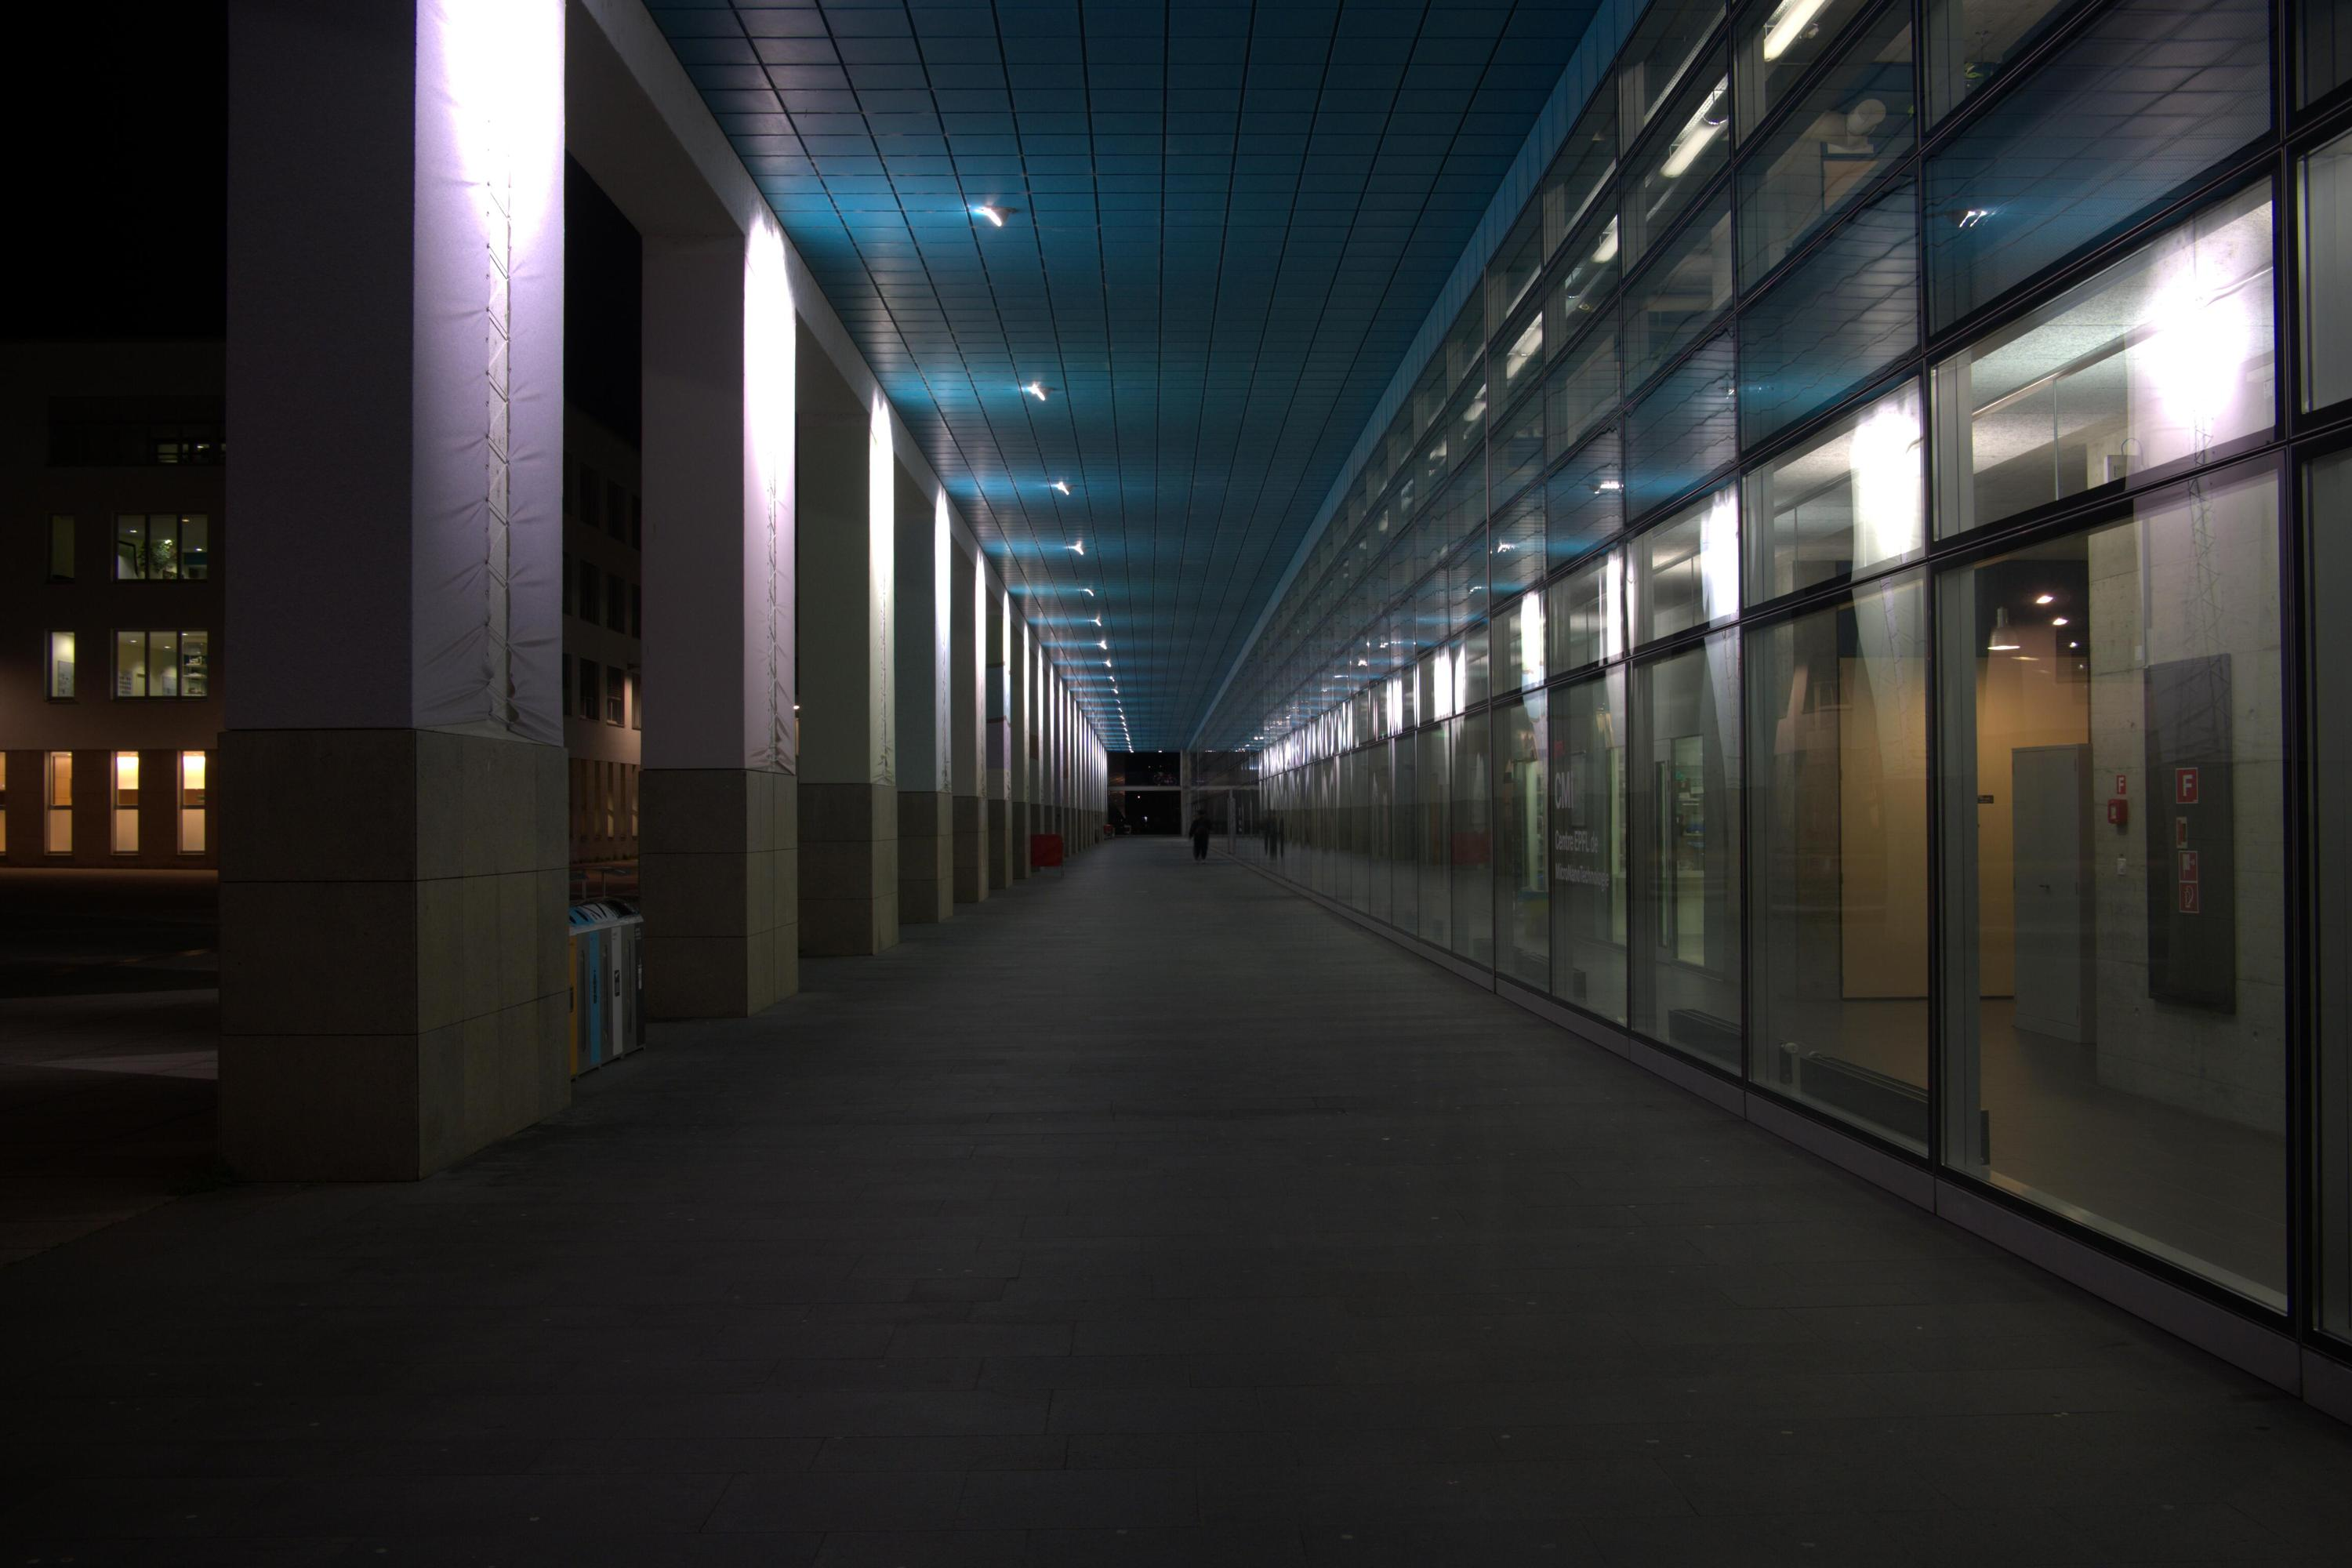
\includegraphics[width=\linewidth]{figures/digital1.jpeg}
    \end{subfigure}
    \hfill
    \begin{subfigure}[t]{.19\textwidth}
      \centering
      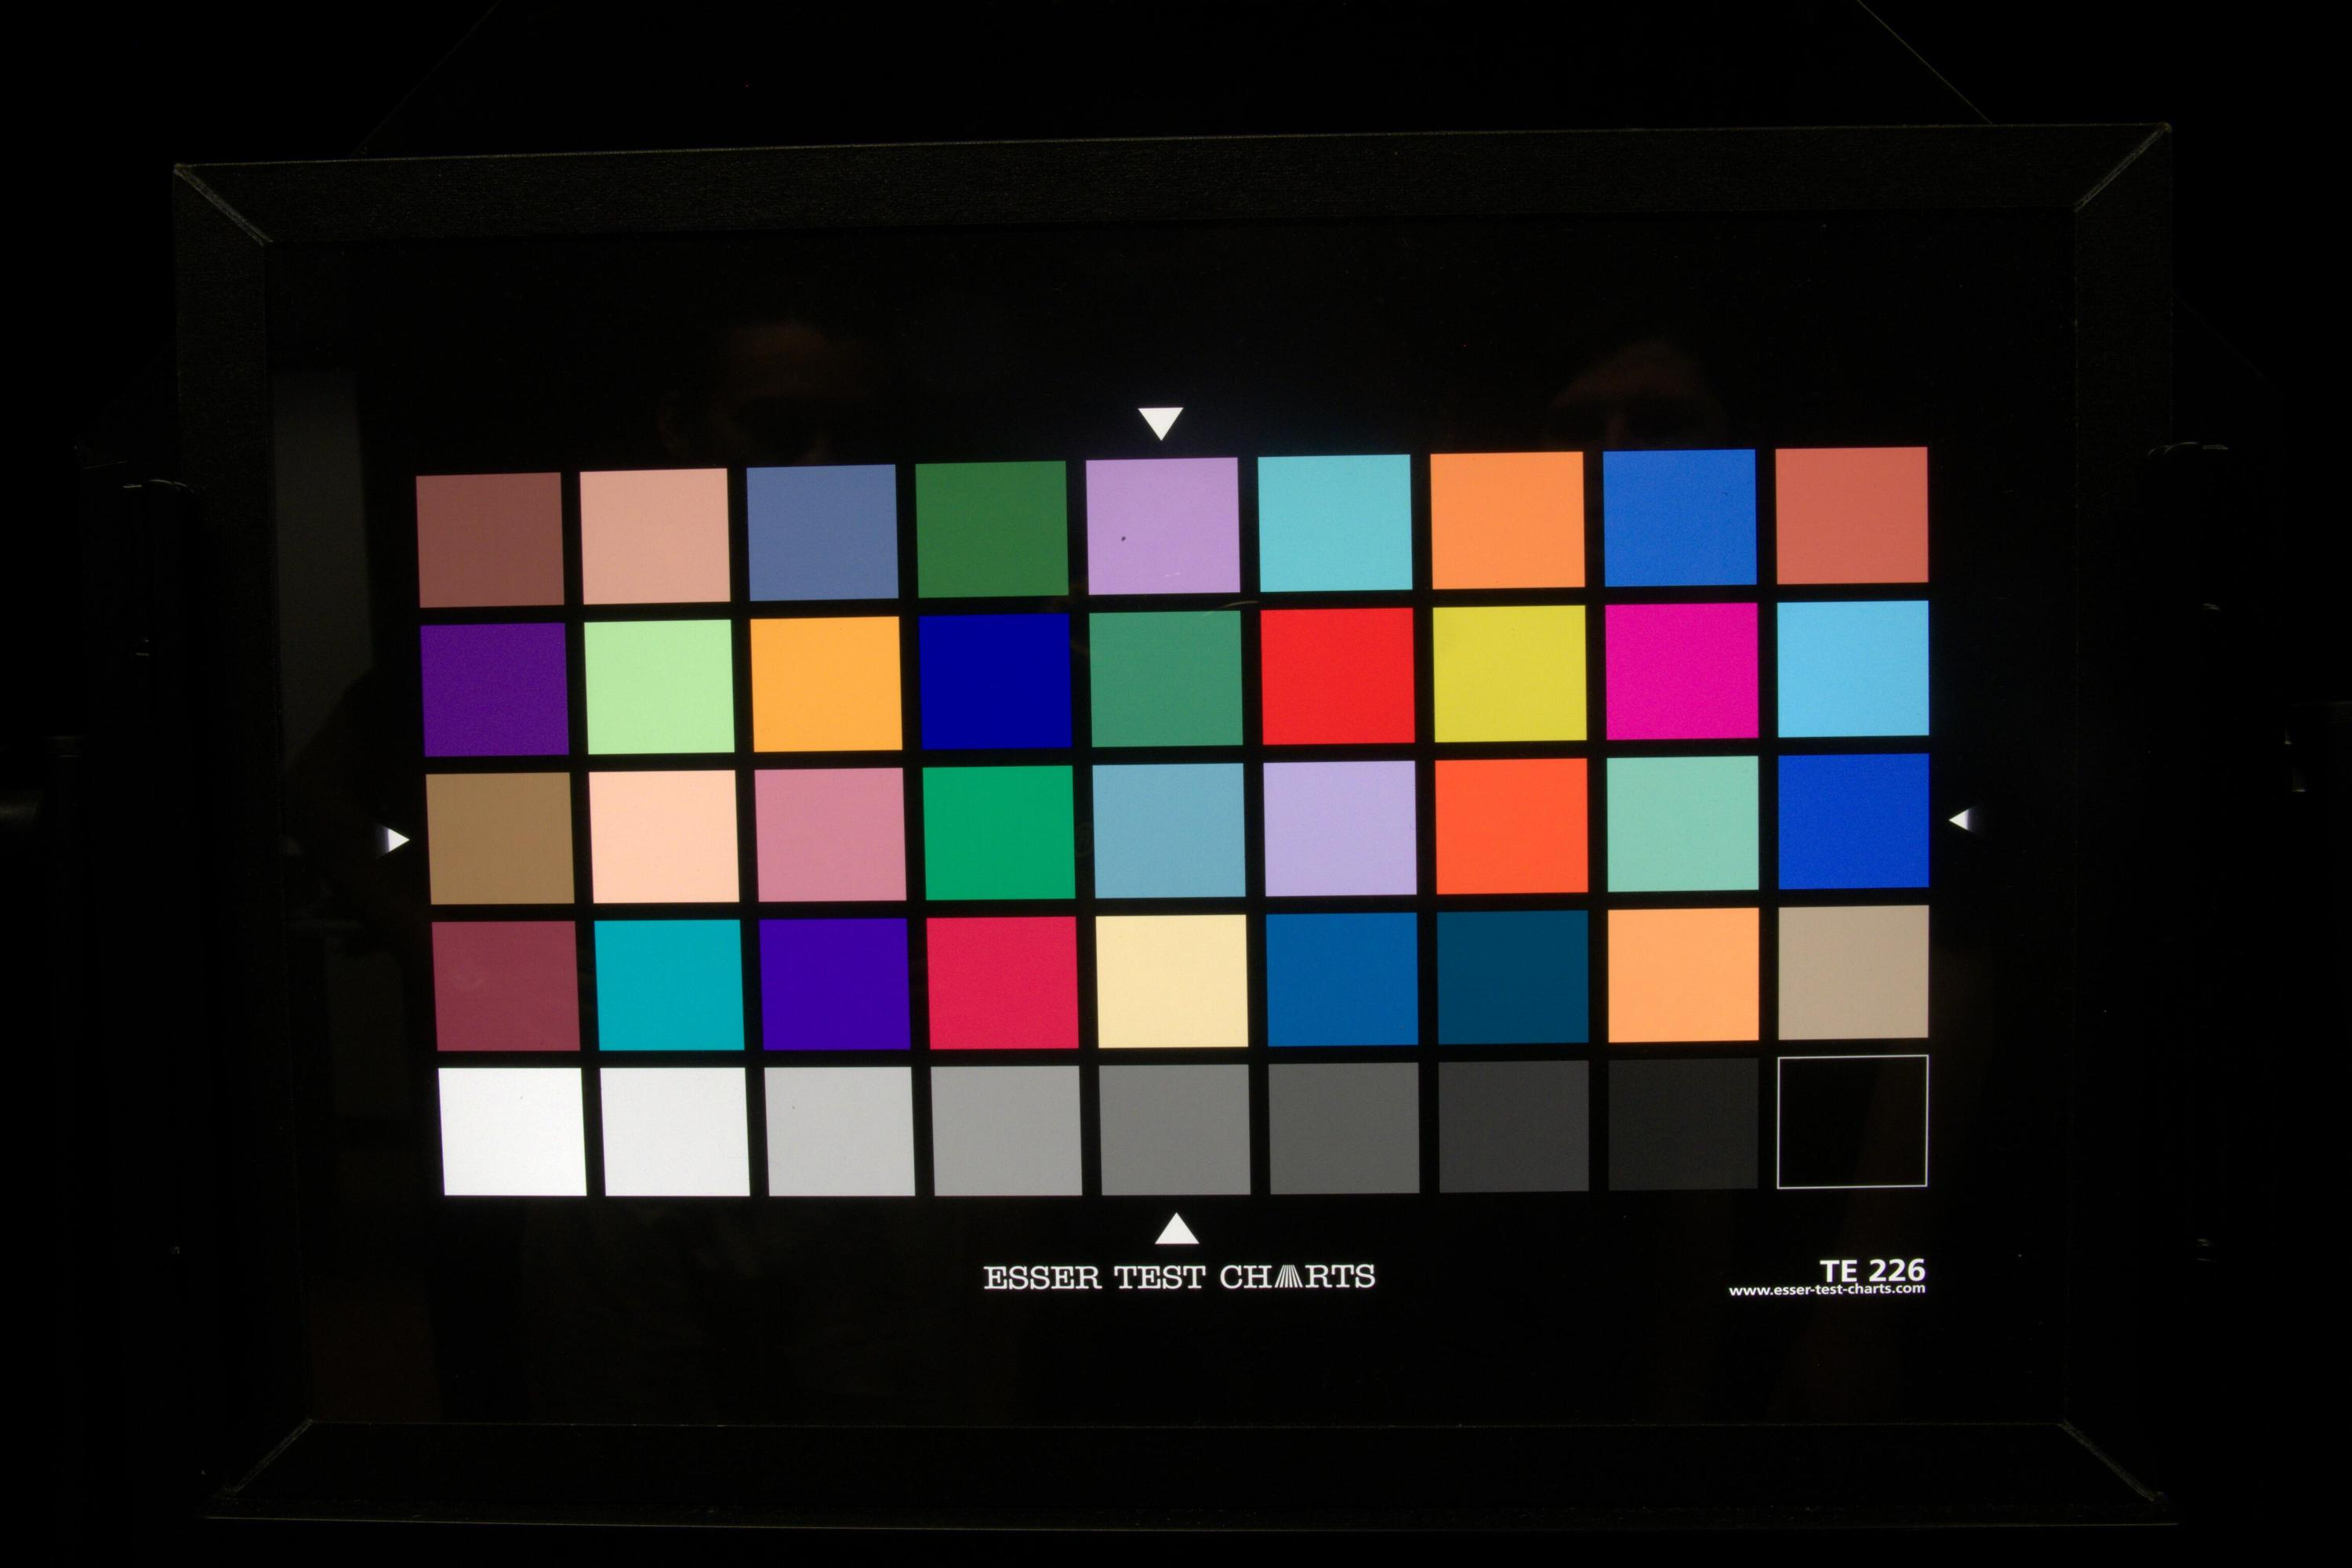
\includegraphics[width=\linewidth]{figures/digital2.jpeg}
    \end{subfigure}
    \hfill
    \begin{subfigure}[t]{.19\textwidth}
      \centering
      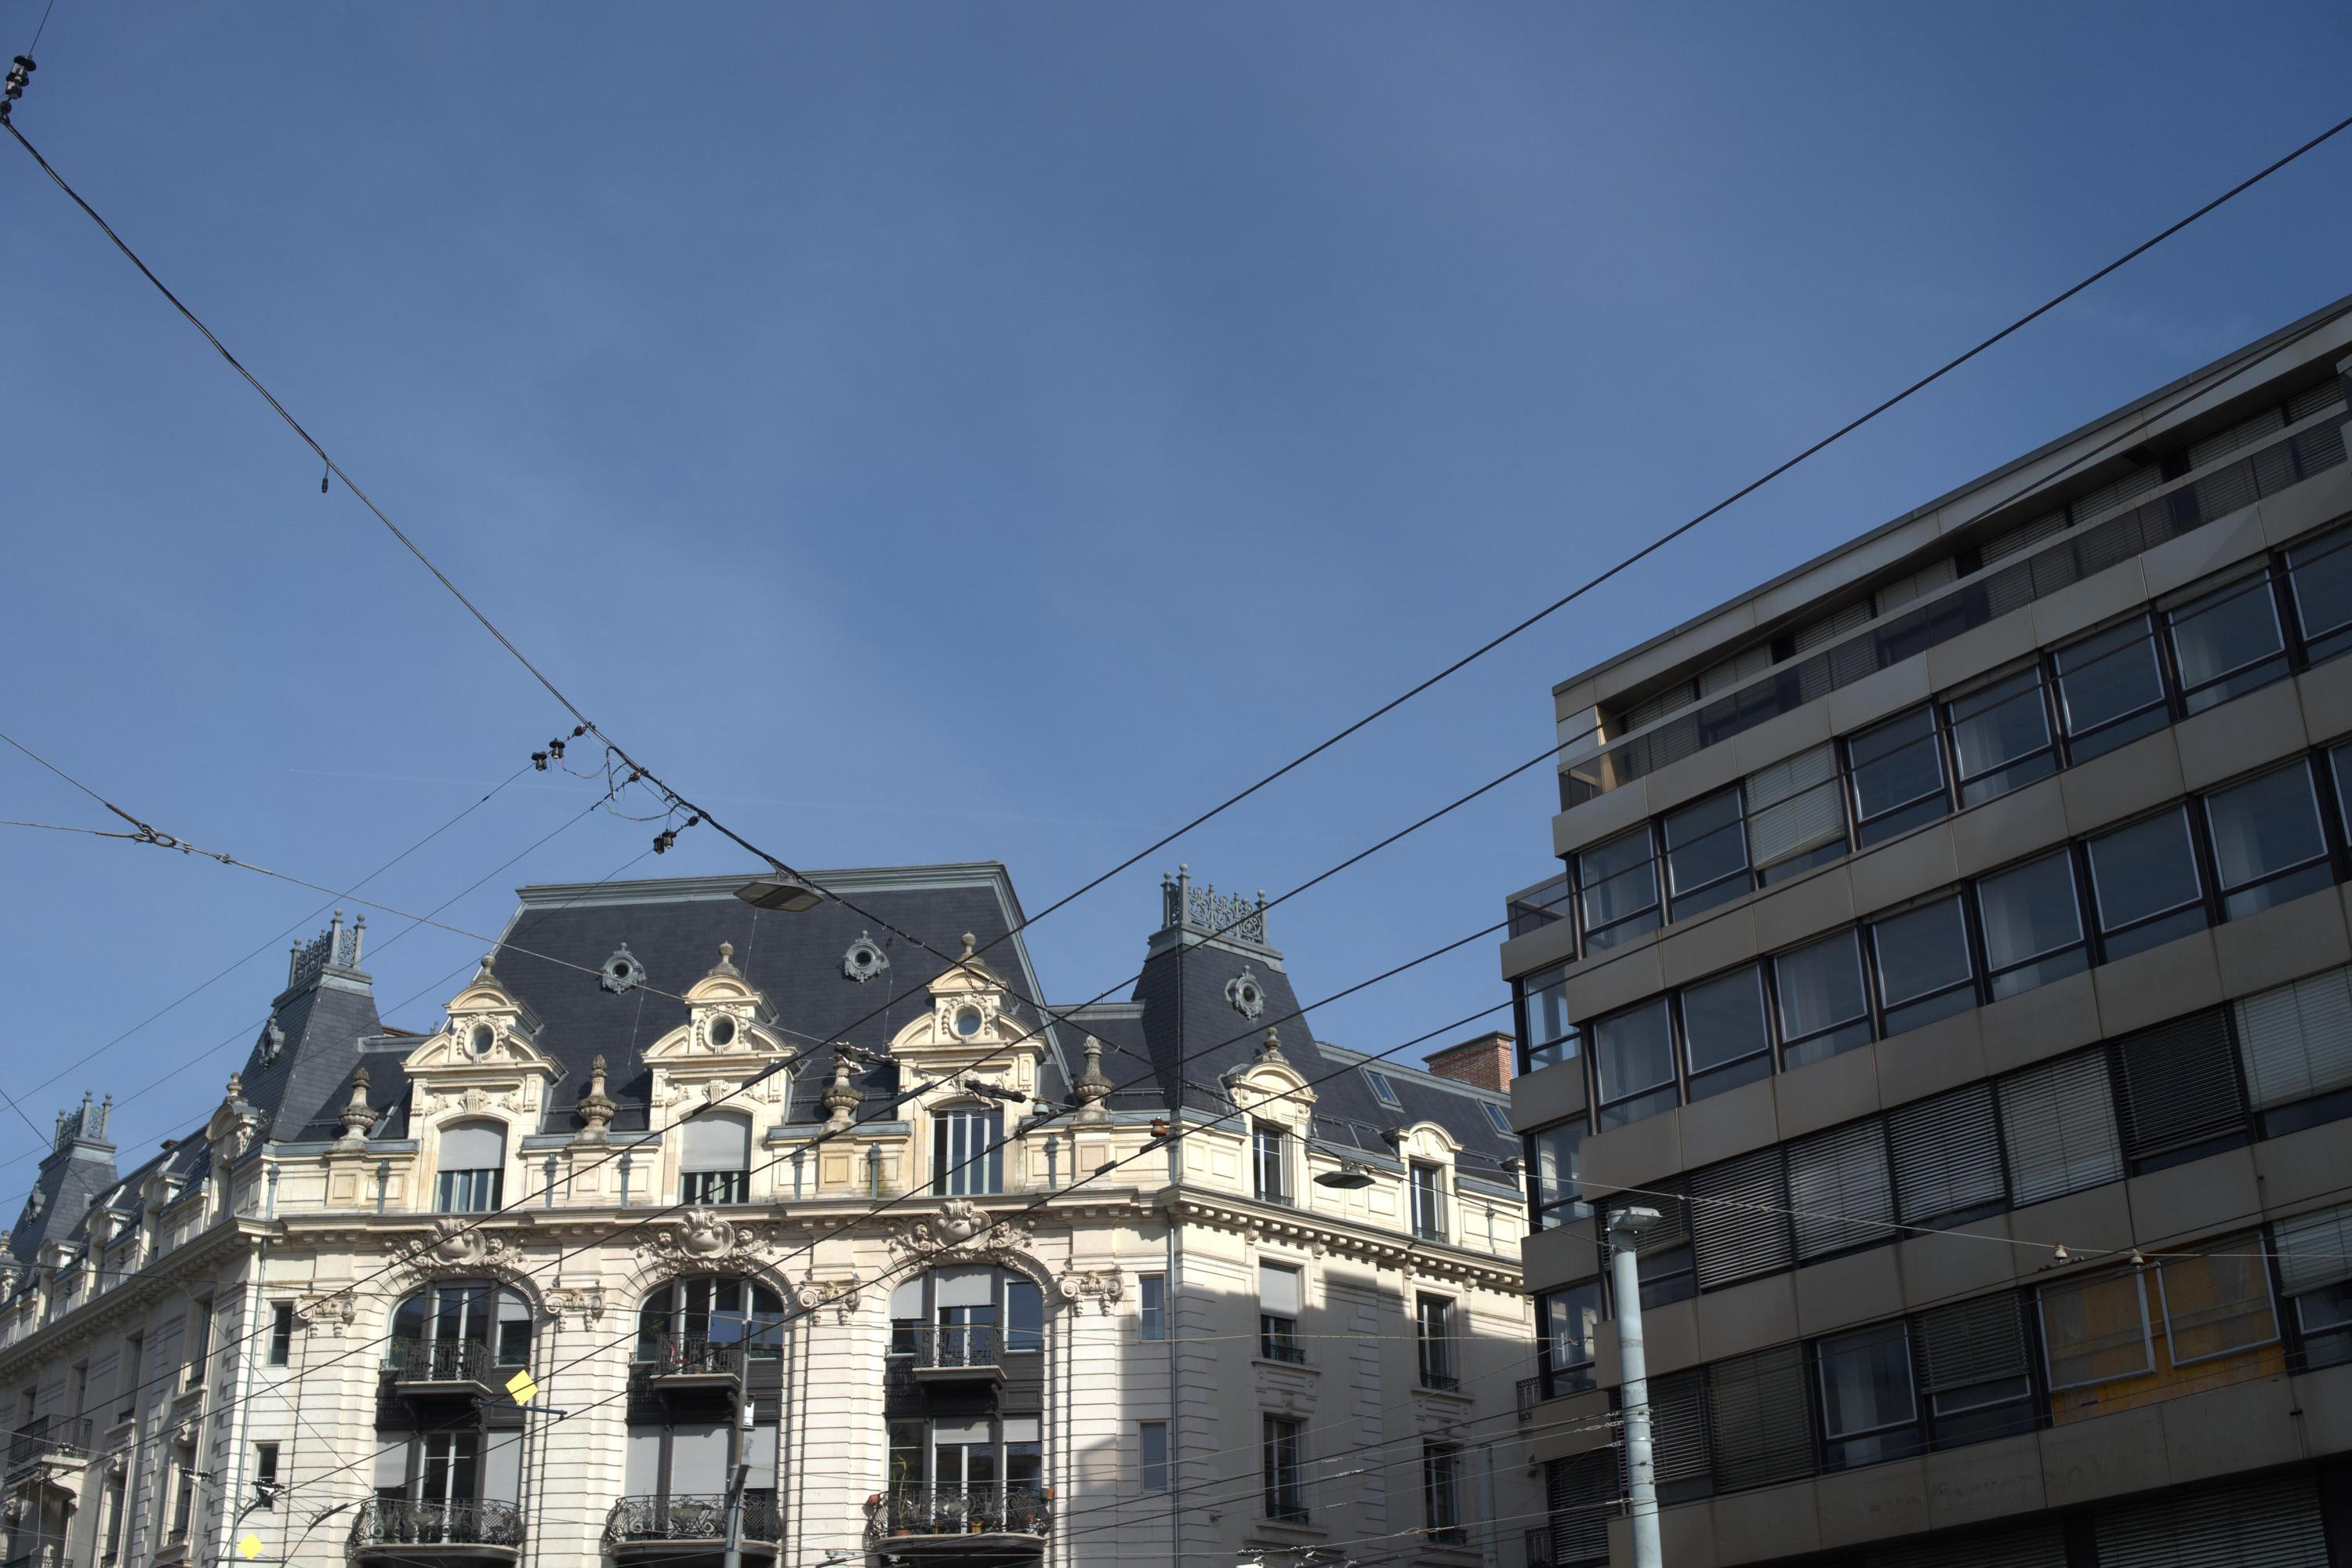
\includegraphics[width=\linewidth]{figures/digital3.jpeg}
    \end{subfigure}
    \hfill
    \begin{subfigure}[t]{.19\textwidth}
      \centering
      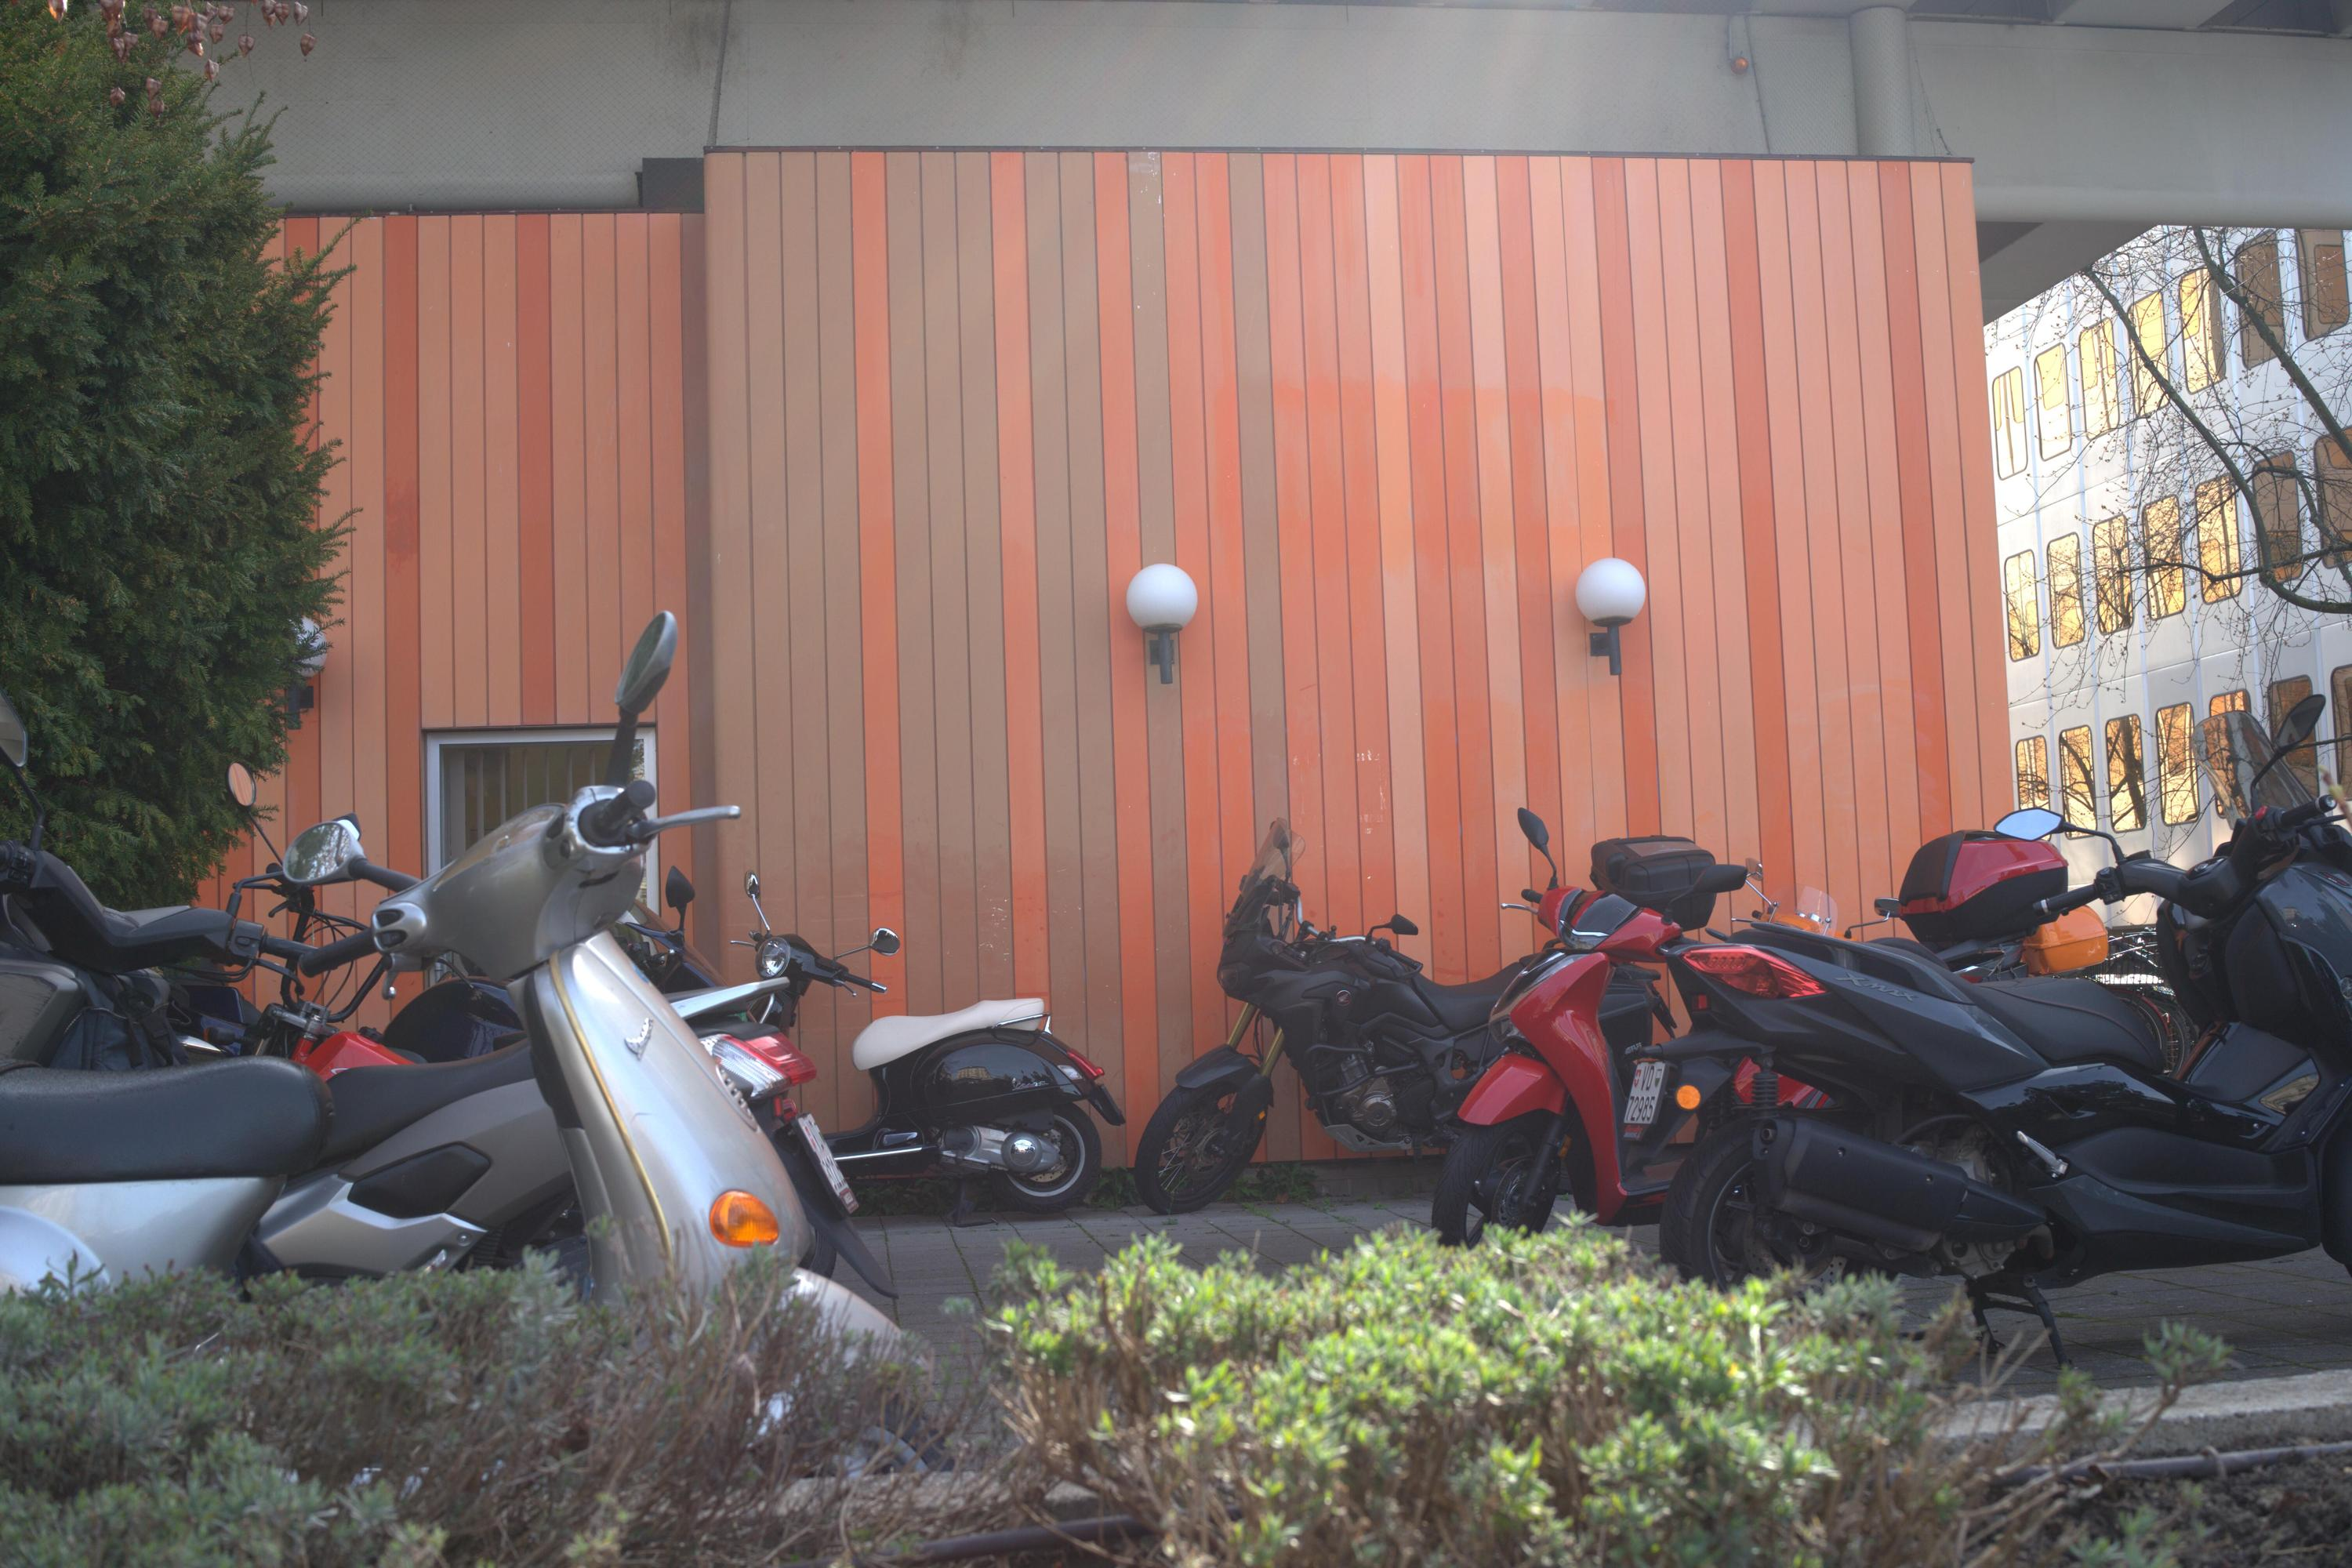
\includegraphics[width=\linewidth]{figures/digital4.jpeg}
    \end{subfigure}
    \begin{subfigure}[t]{.19\textwidth}
      \centering
      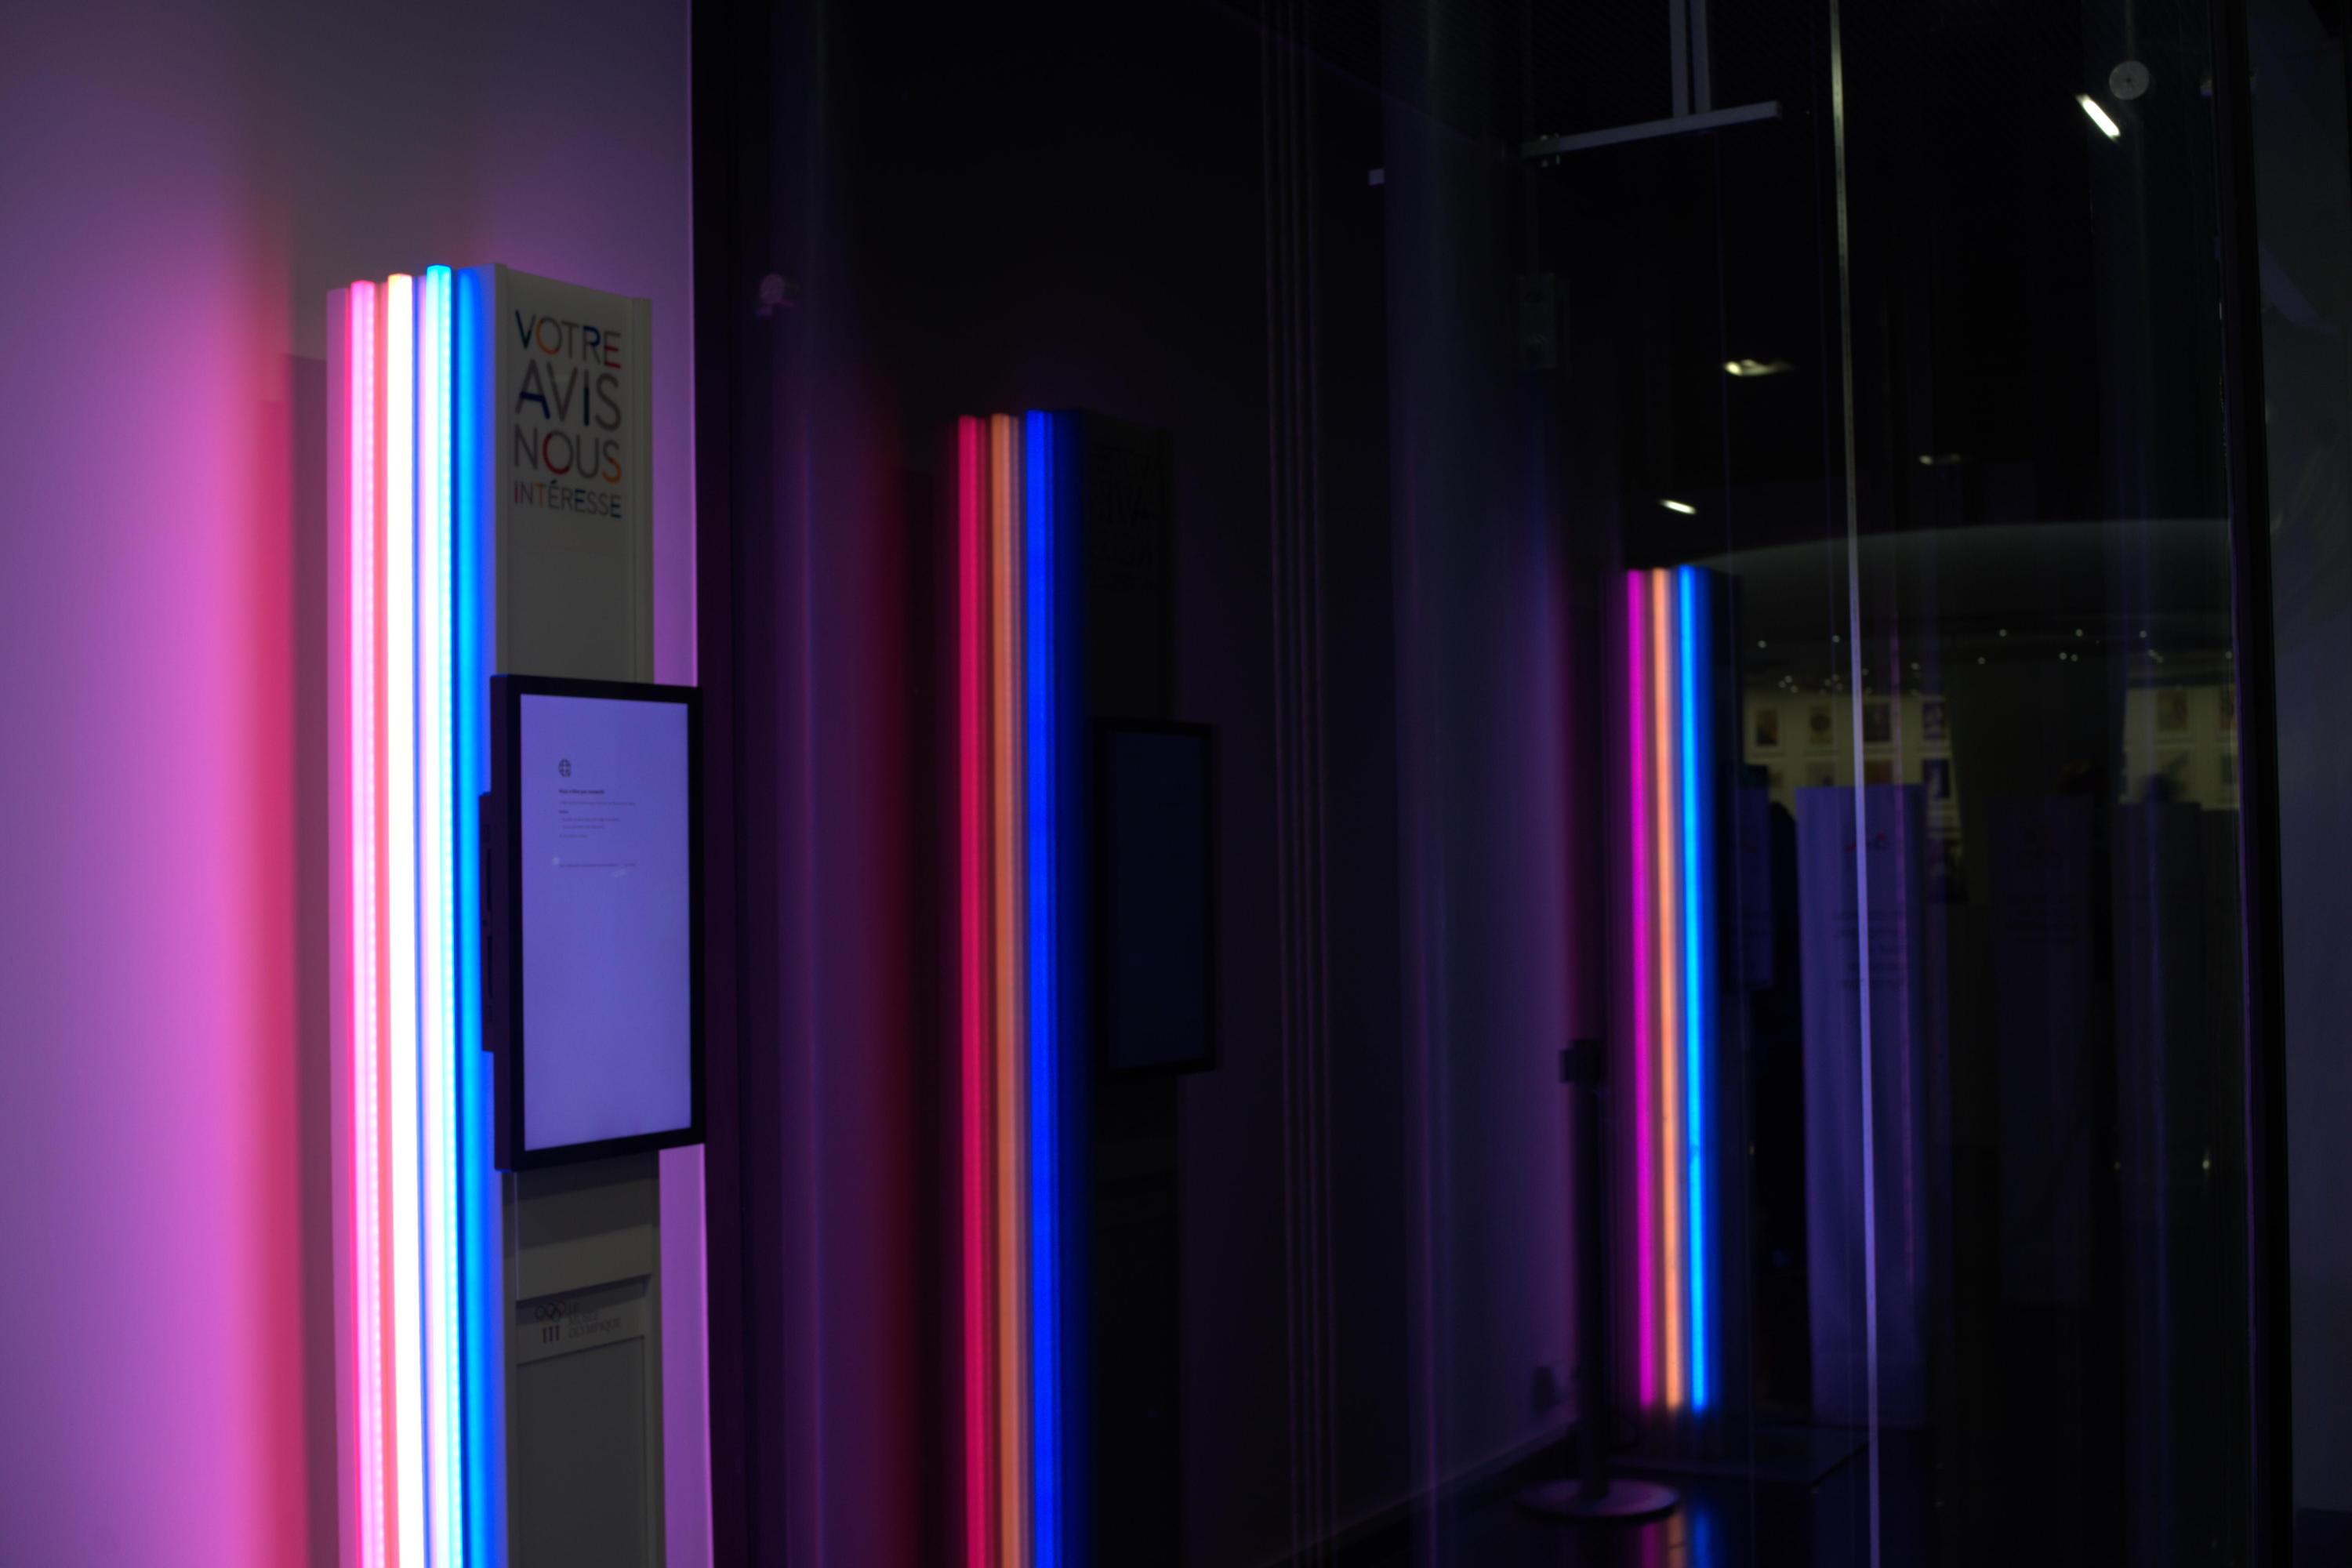
\includegraphics[width=\linewidth]{figures/digital5.jpeg}
    \end{subfigure}
  
    \medskip

    \begin{subfigure}[t]{.19\textwidth}
      \centering
      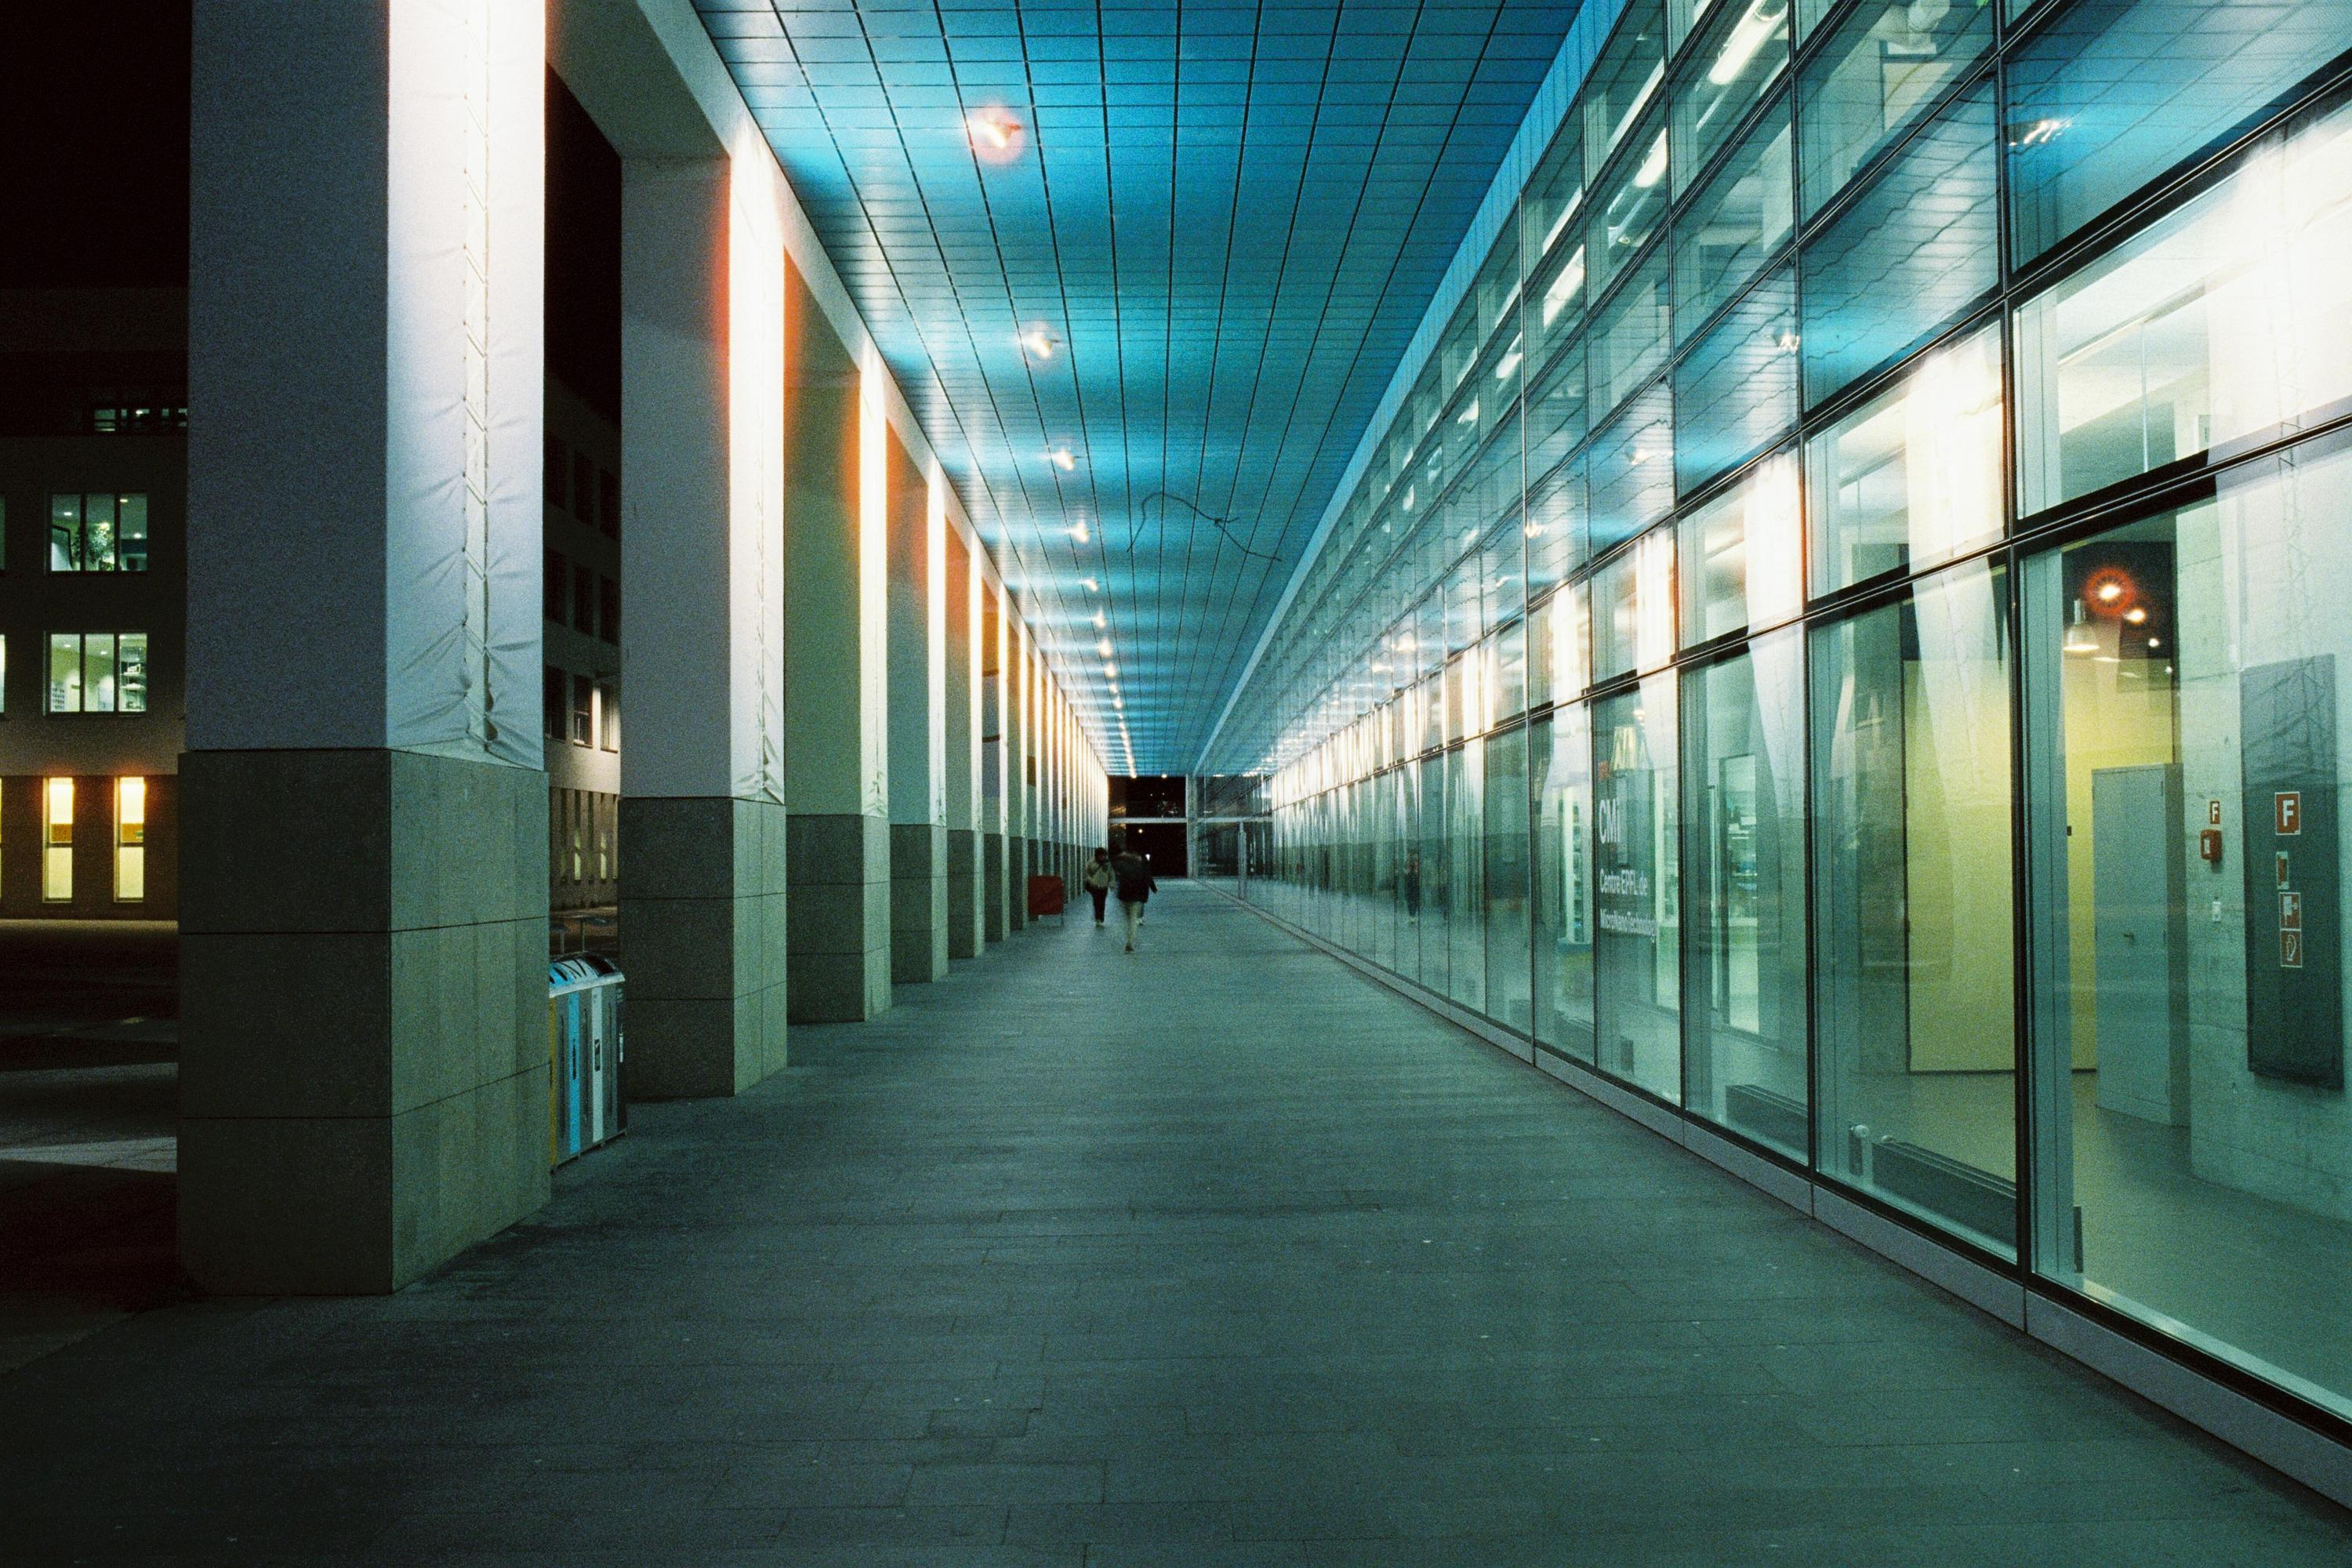
\includegraphics[width=\linewidth]{figures/film1.jpeg}
    \end{subfigure}
    \hfill
    \begin{subfigure}[t]{.19\textwidth}
      \centering
      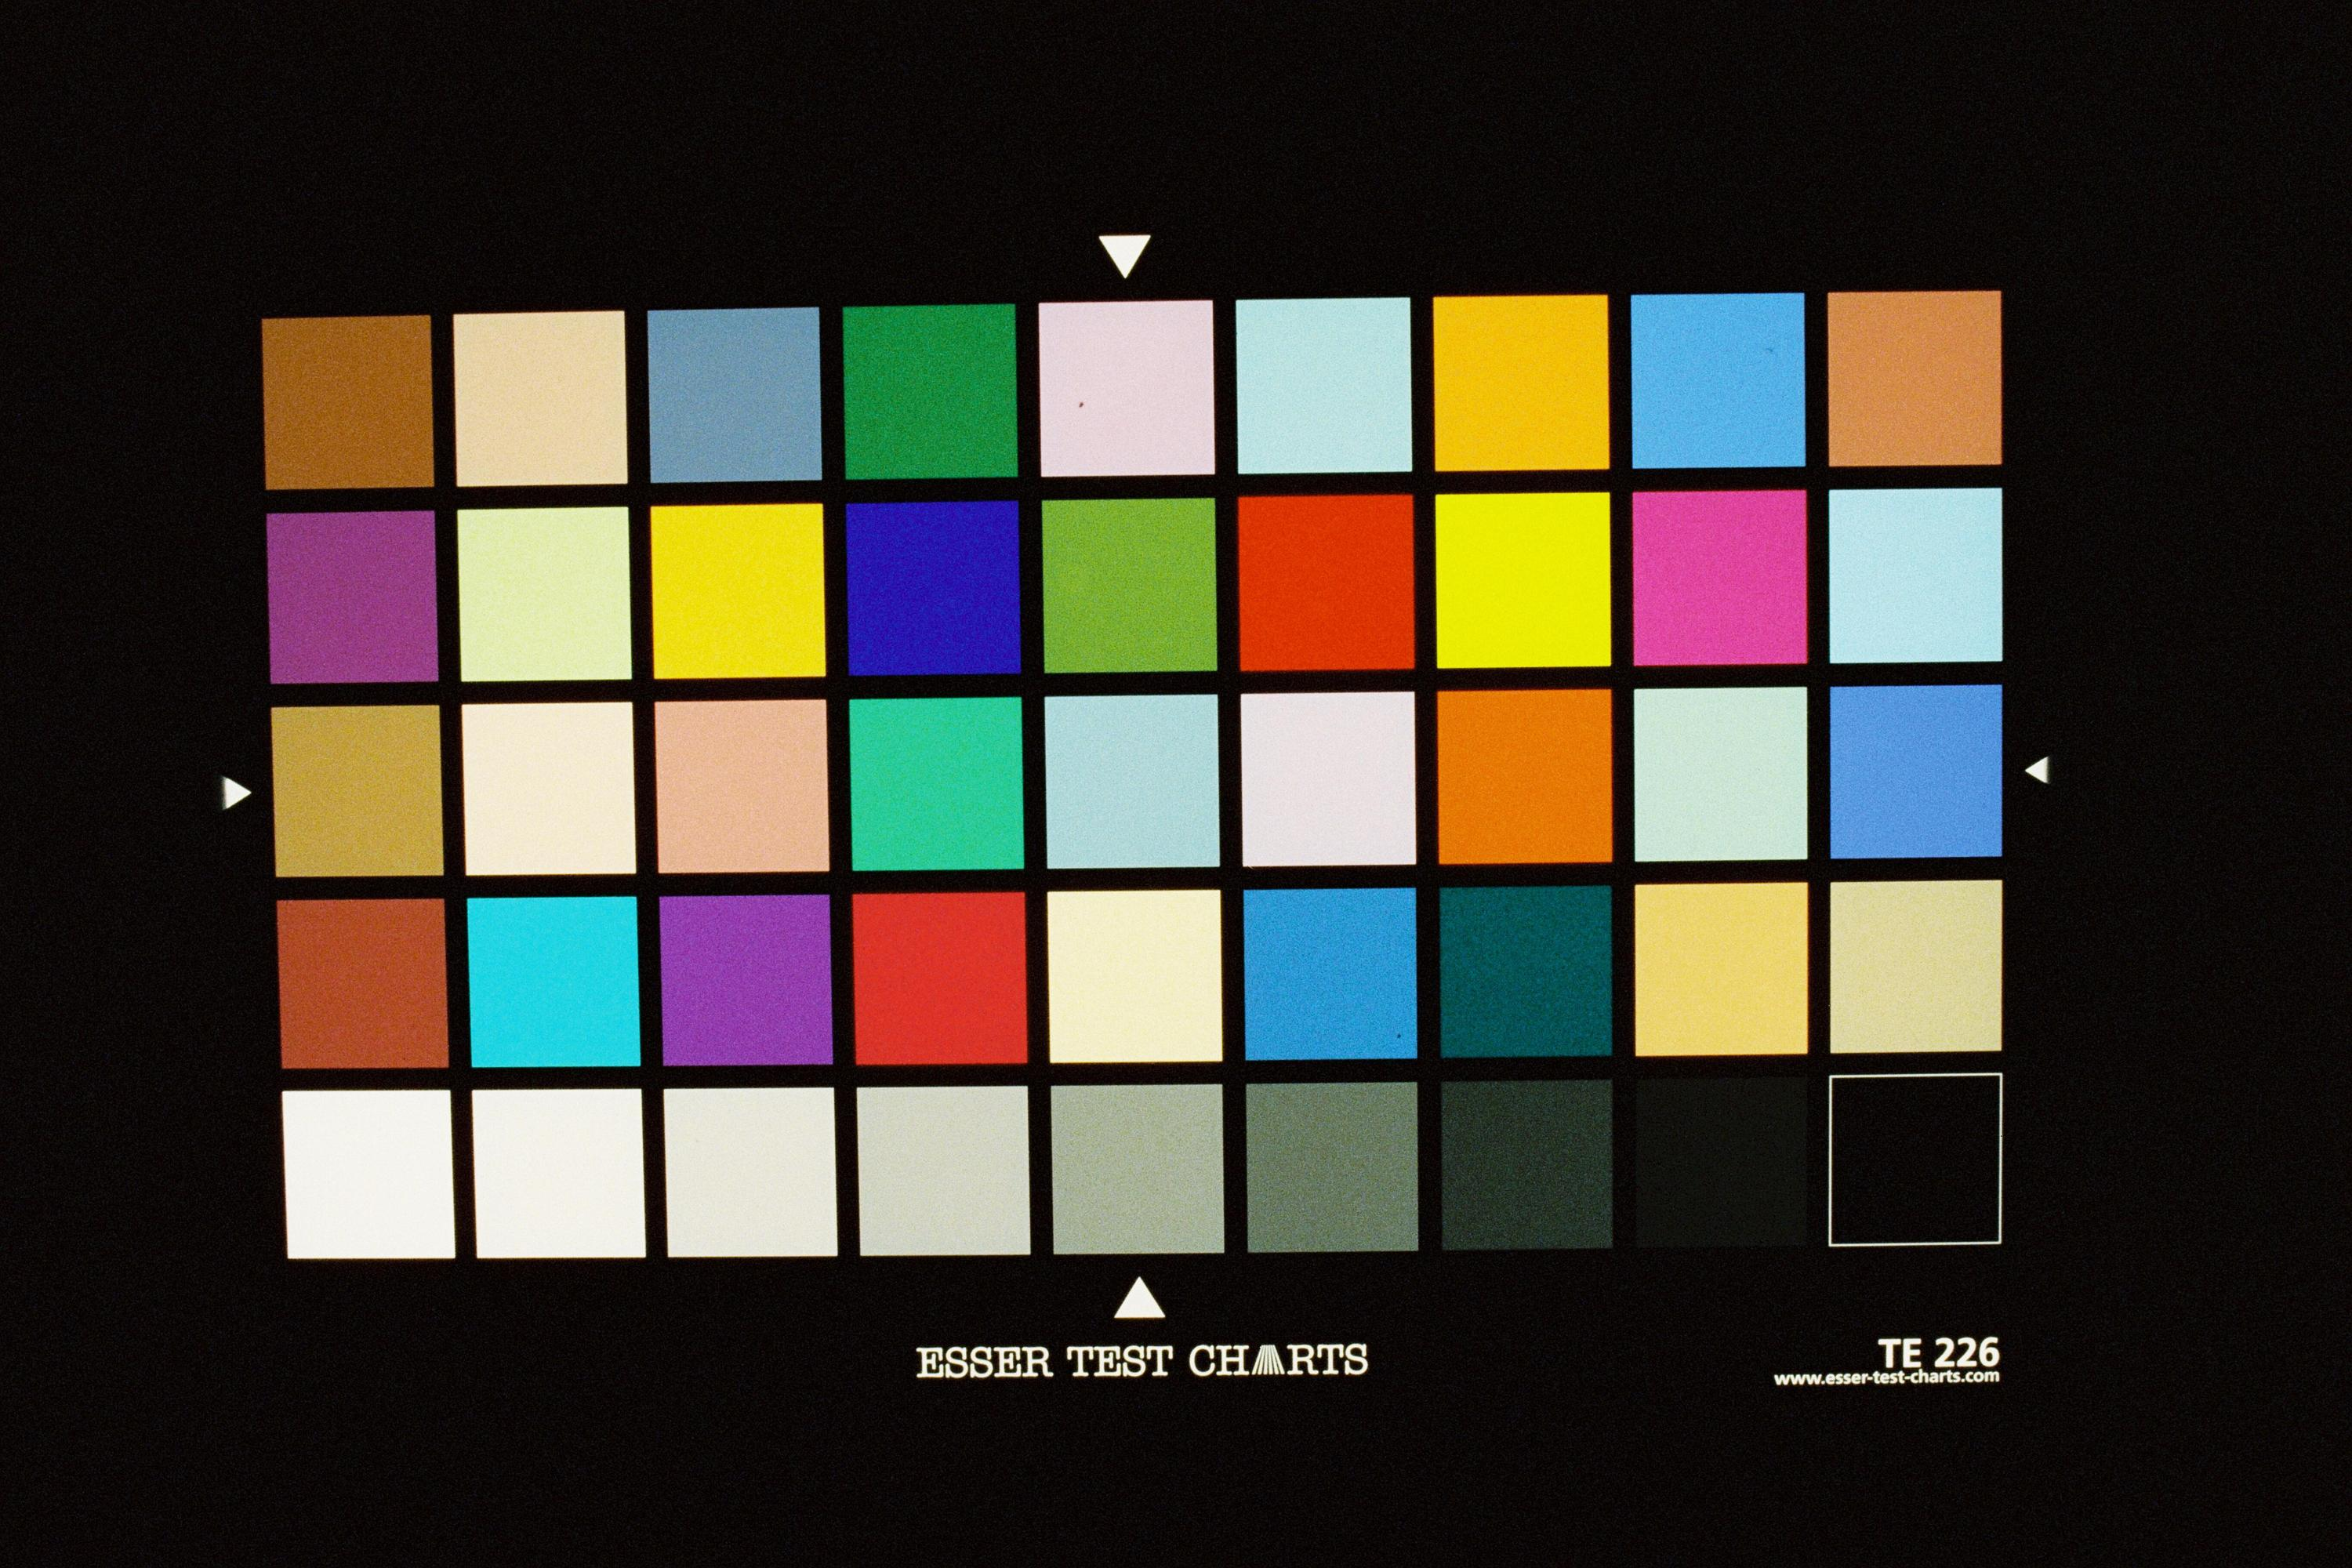
\includegraphics[width=\linewidth]{figures/film2.jpeg}
    \end{subfigure}
    \hfill
    \begin{subfigure}[t]{.19\textwidth}
      \centering
      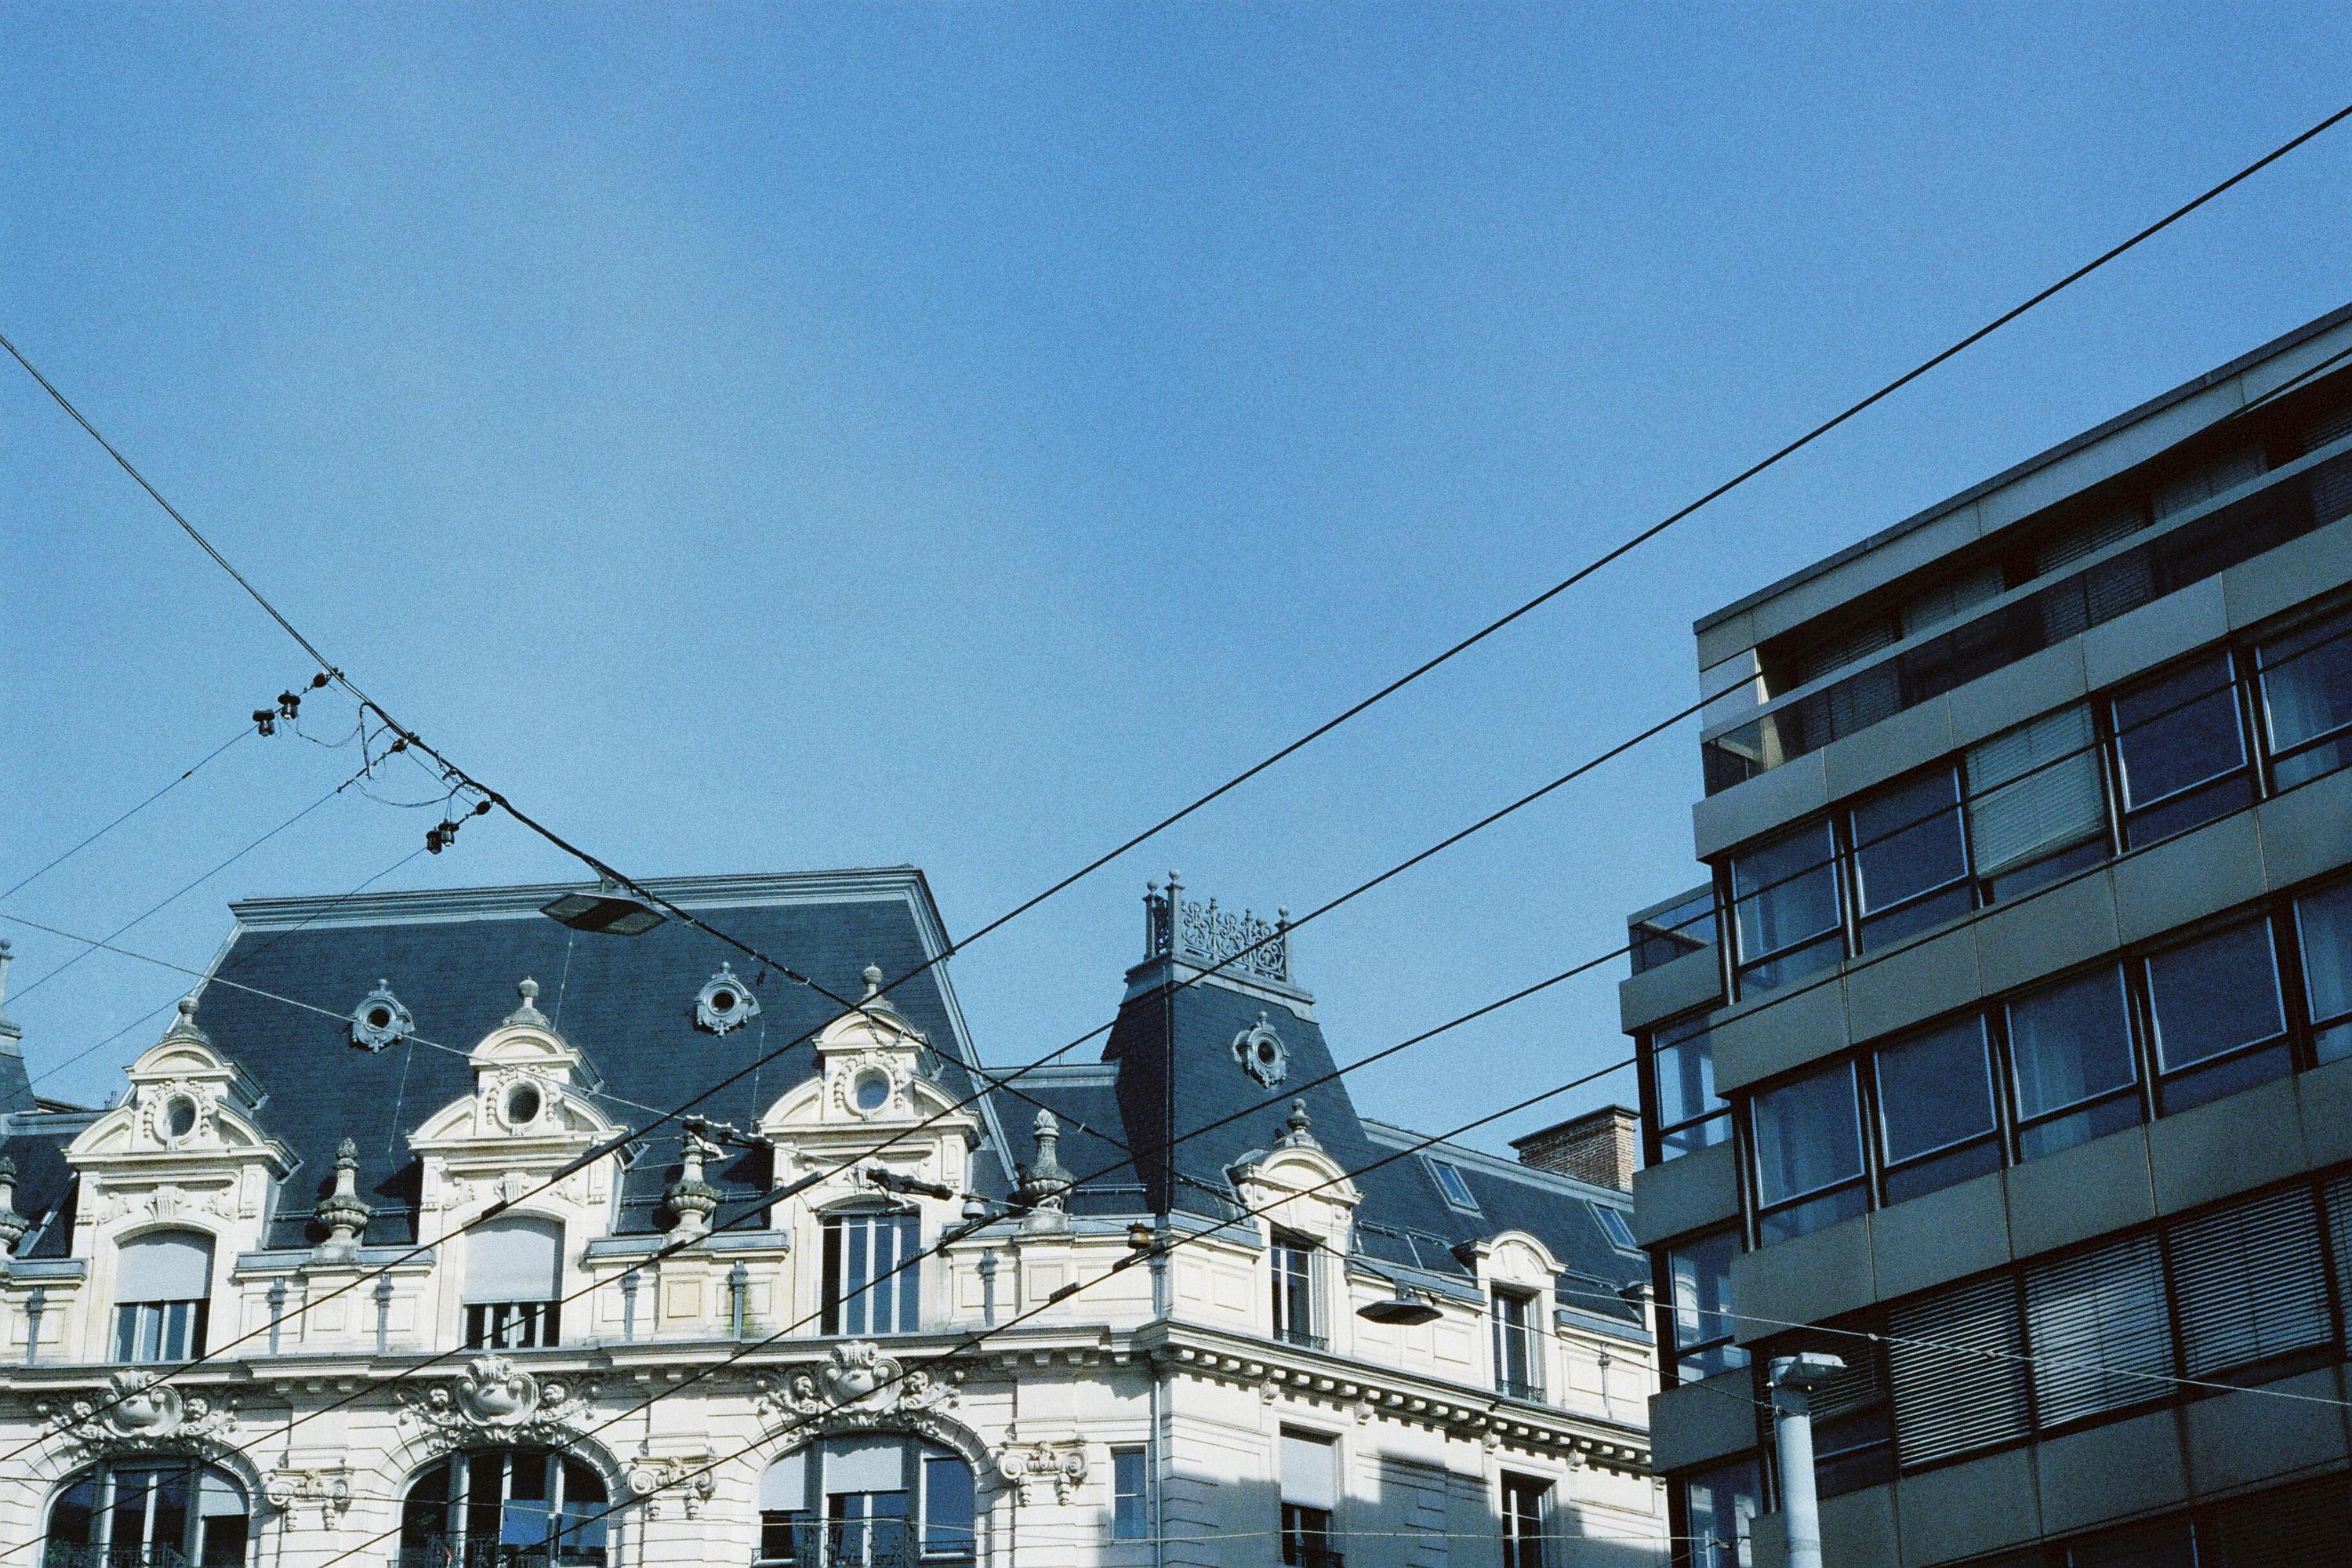
\includegraphics[width=\linewidth]{figures/film3.jpeg}
    \end{subfigure}
    \hfill
    \begin{subfigure}[t]{.19\textwidth}
      \centering
      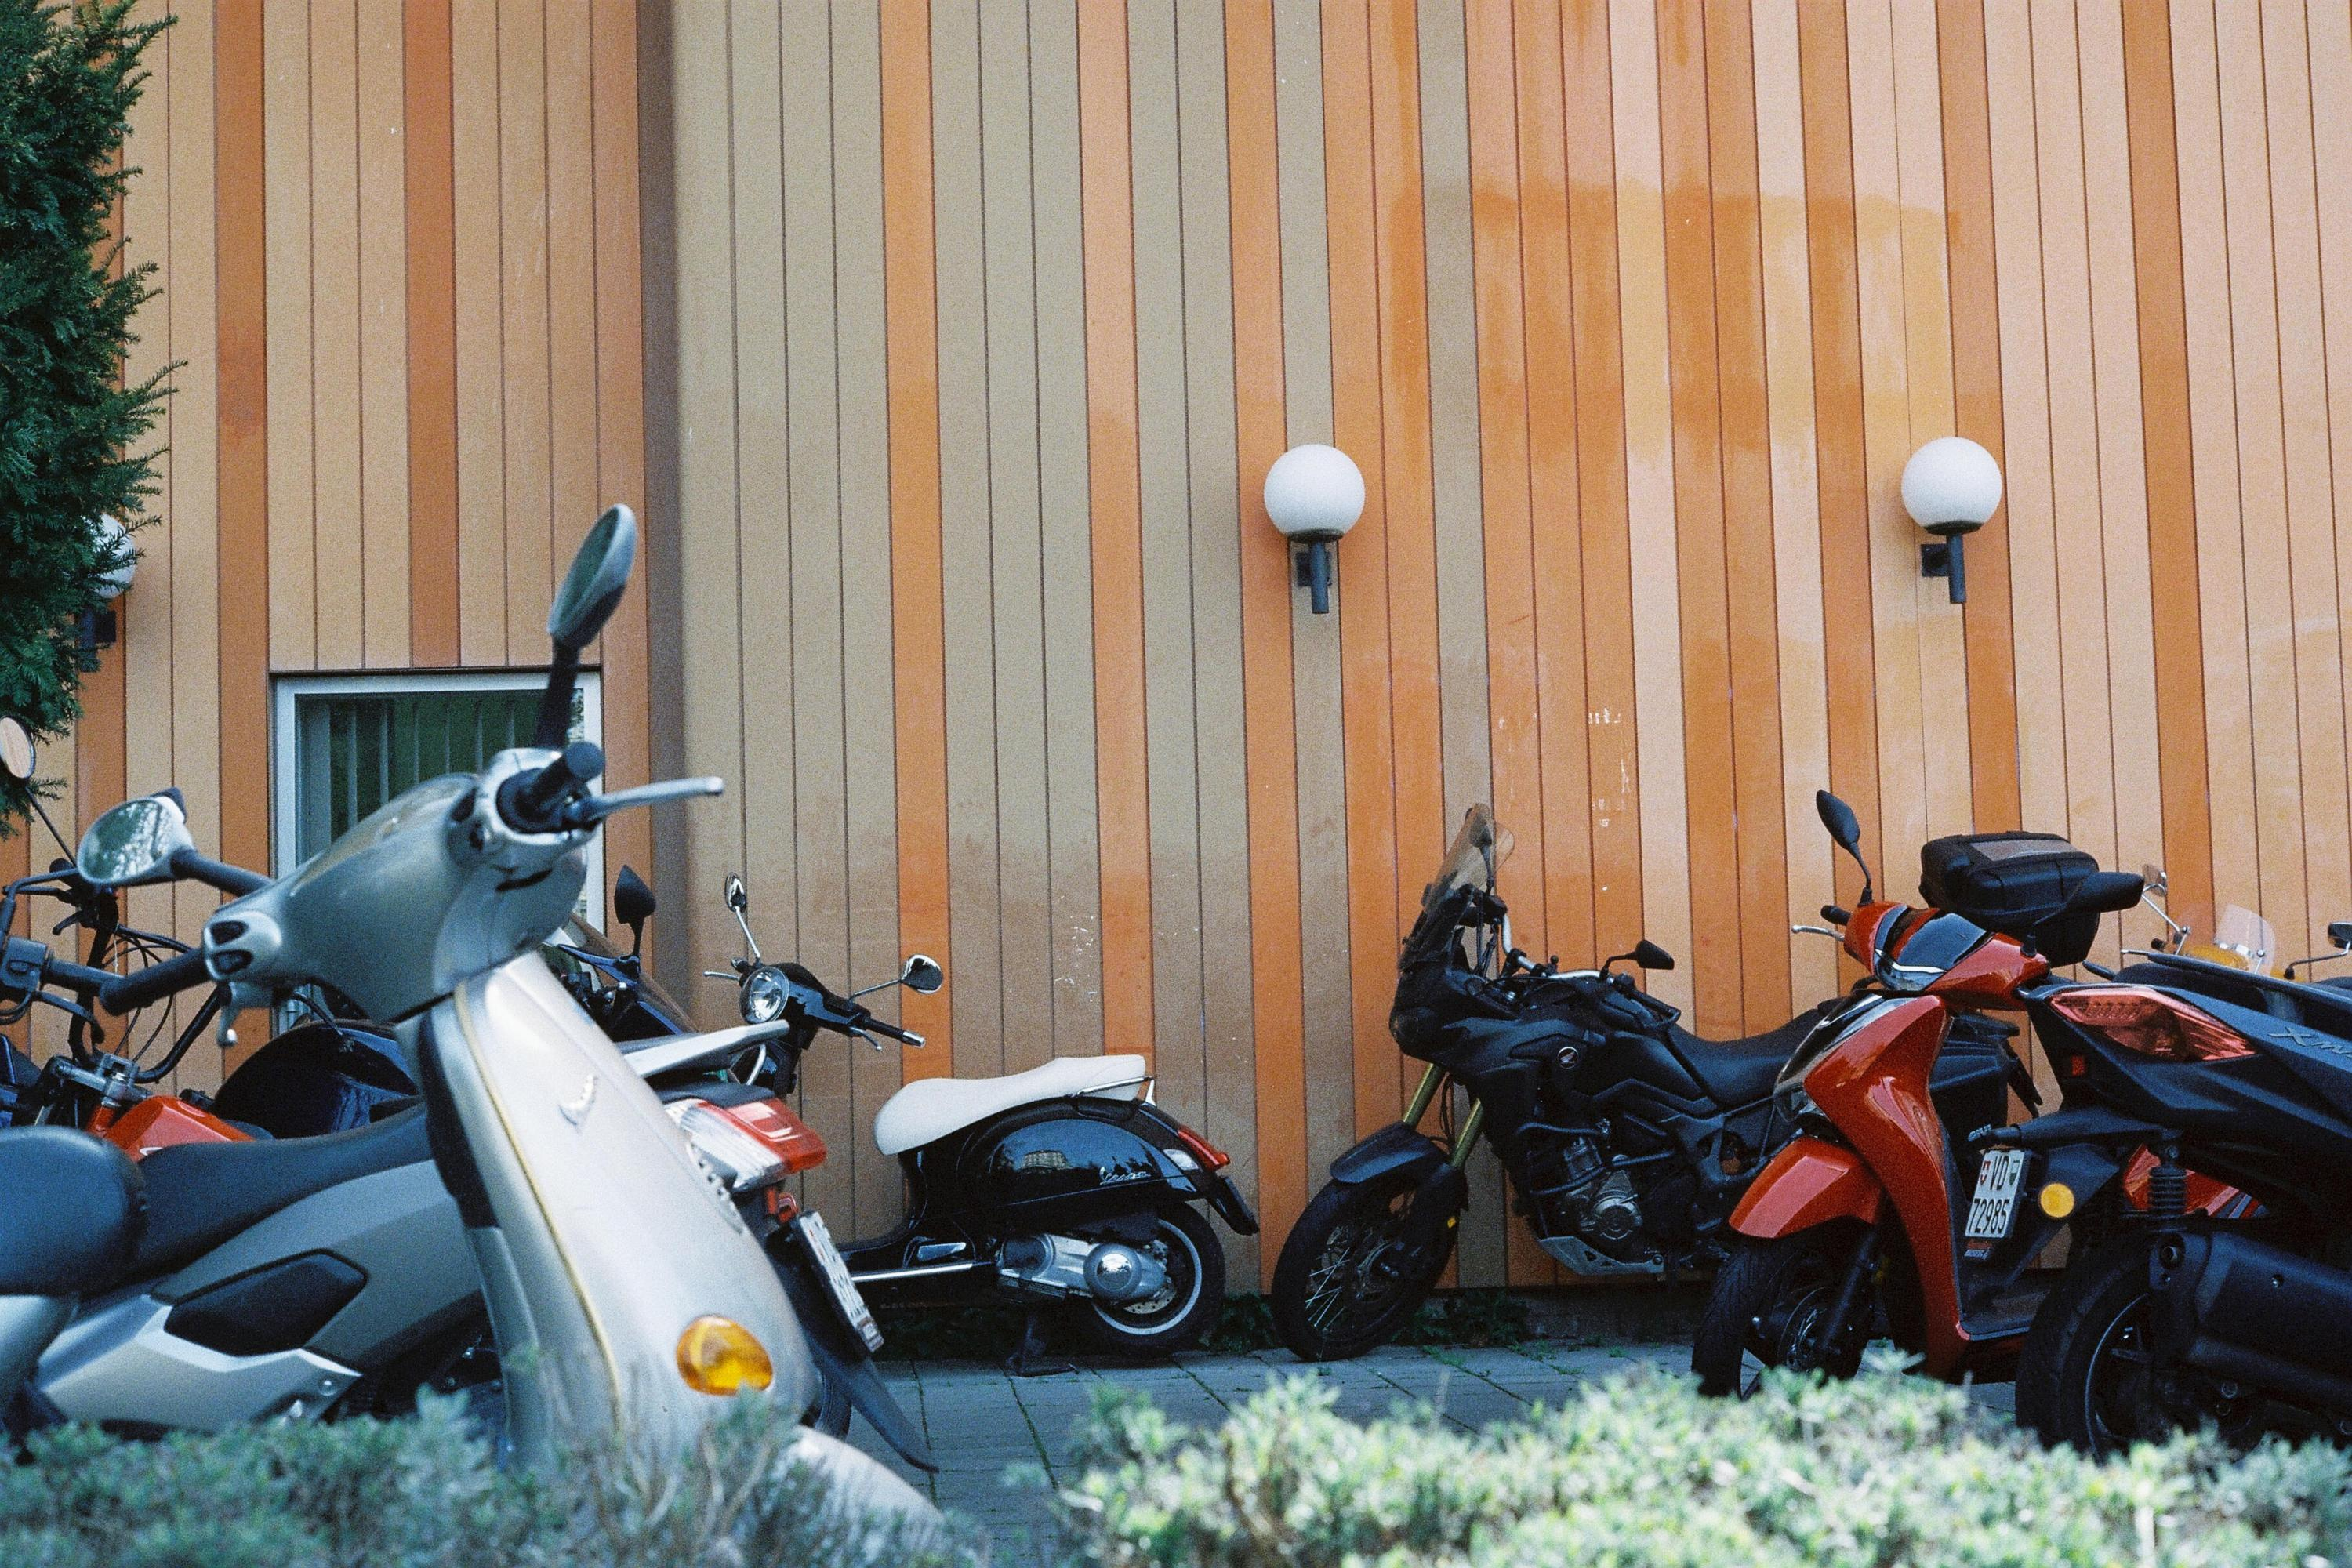
\includegraphics[width=\linewidth]{figures/film4.jpeg}
    \end{subfigure}
    \begin{subfigure}[t]{.19\textwidth}
      \centering
      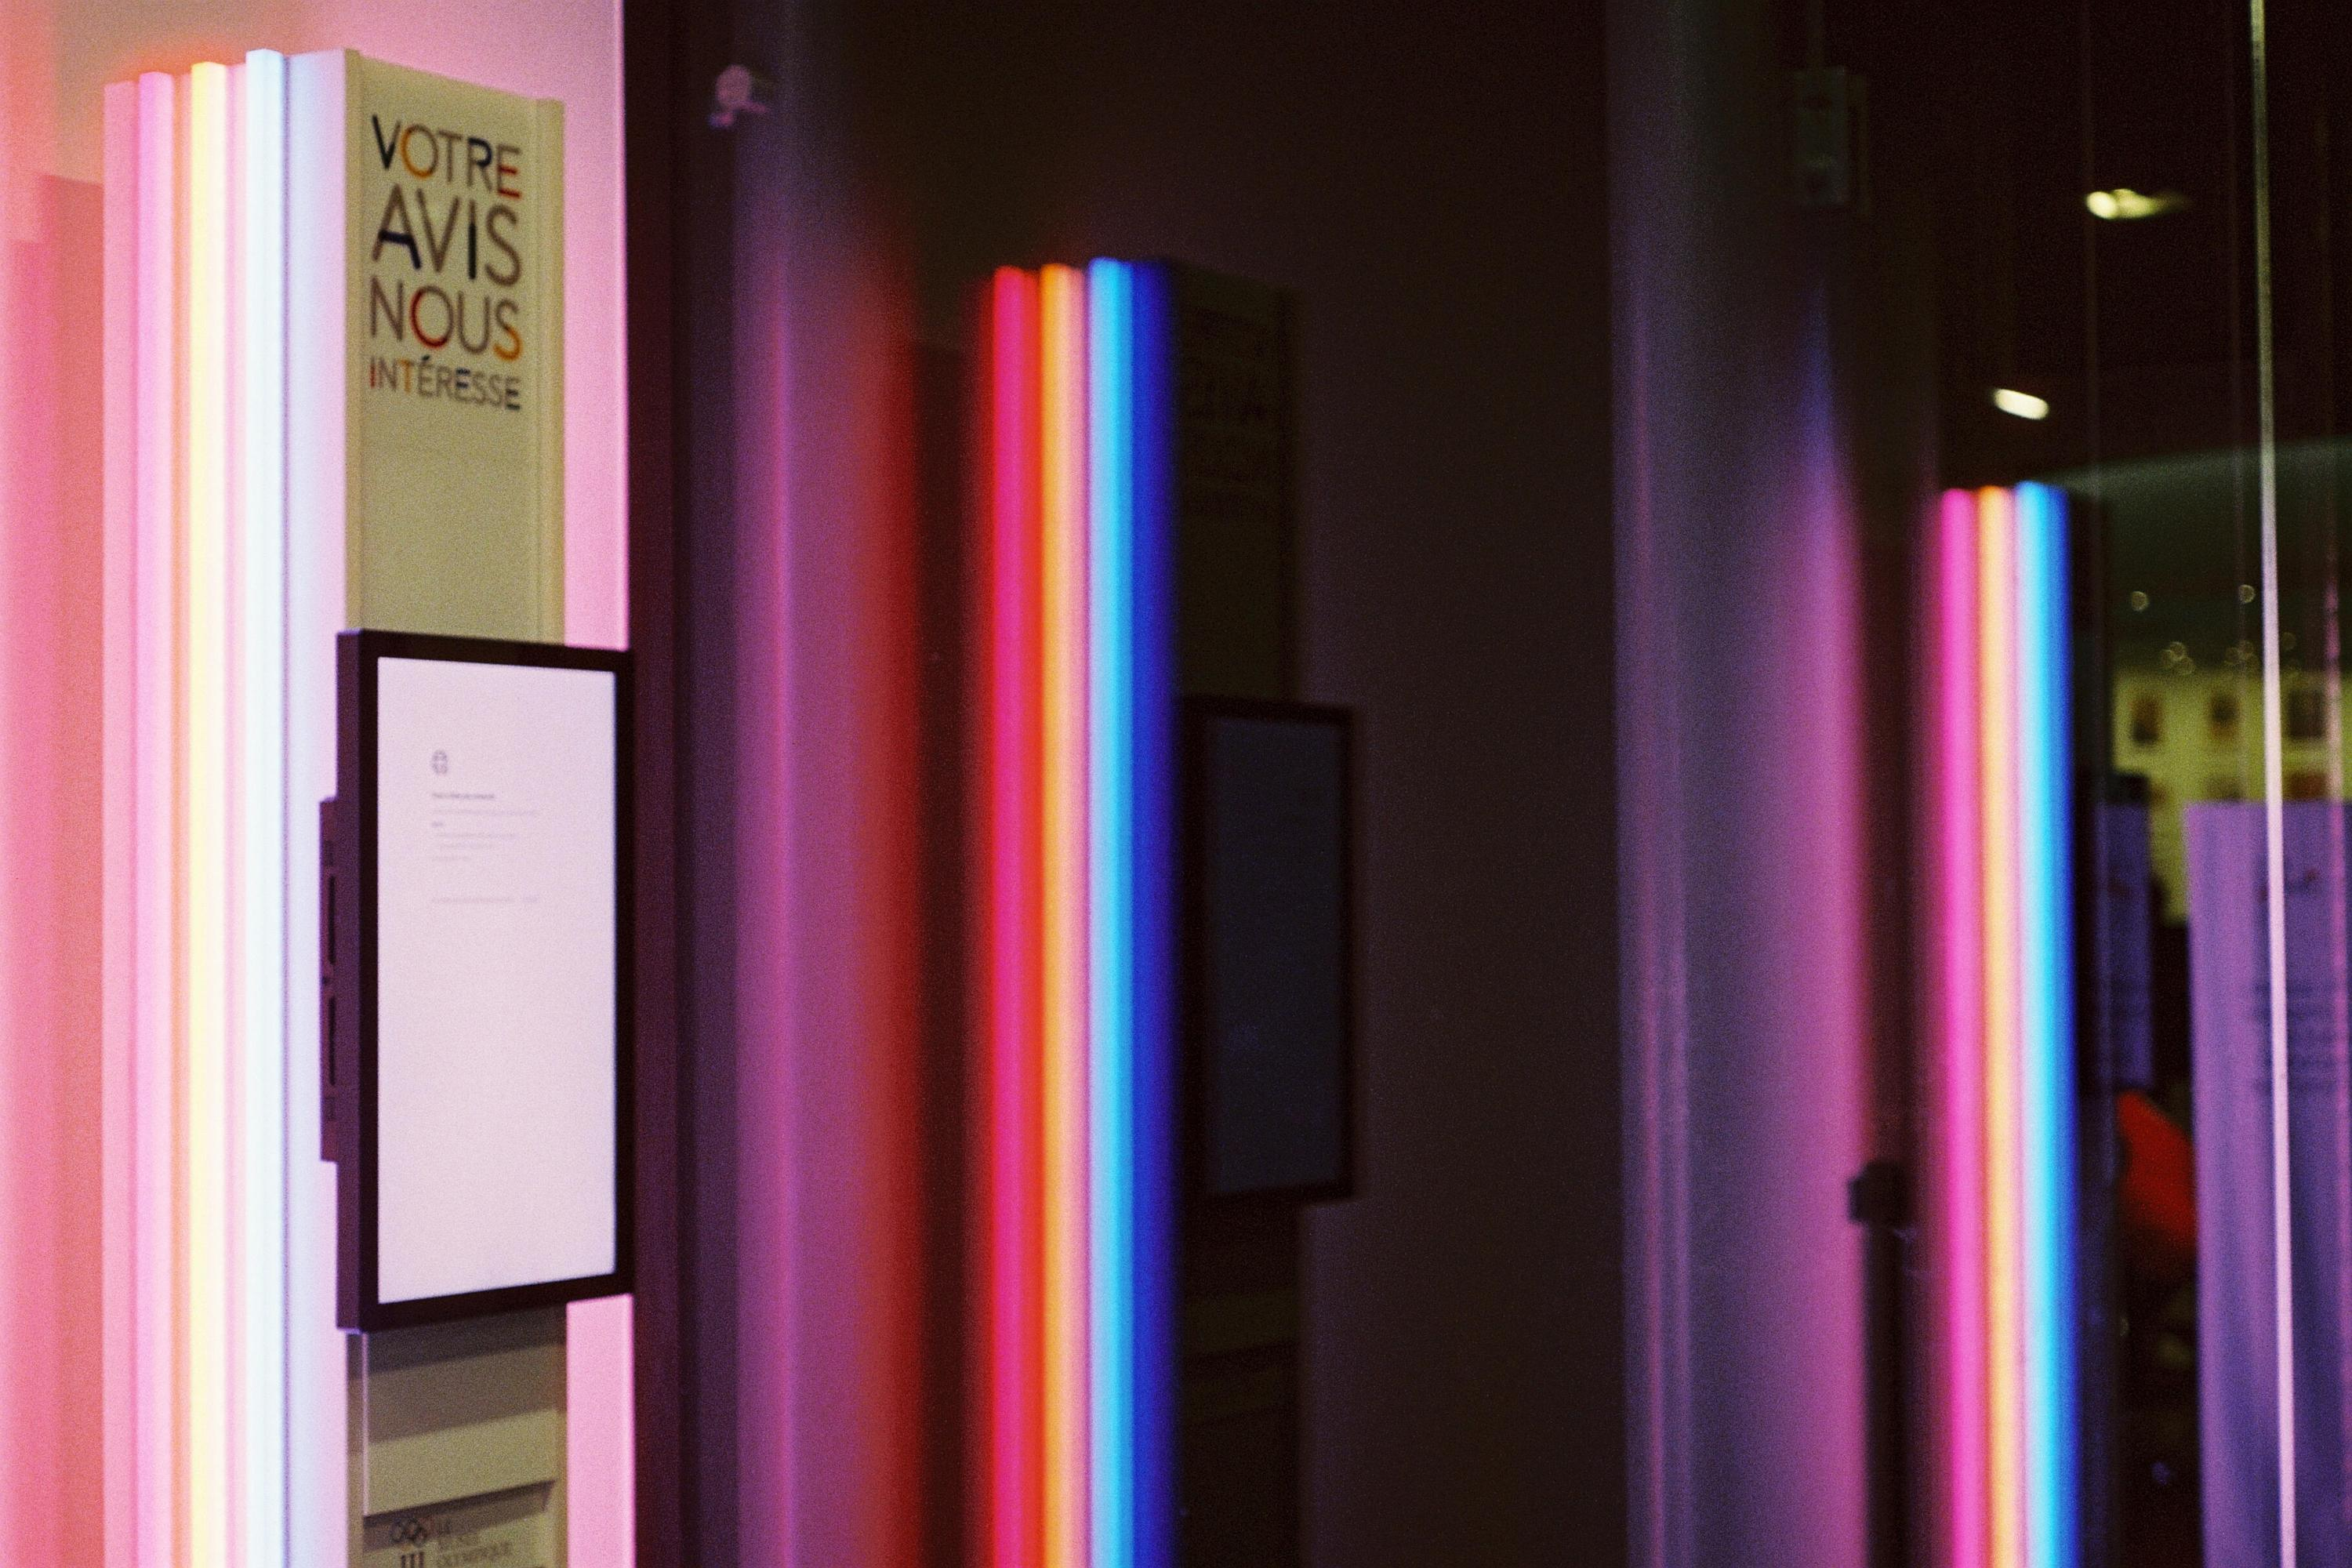
\includegraphics[width=\linewidth]{figures/film5.jpeg}
    \end{subfigure}
  
    \caption{\textbf{Raw Paired Image Dataset.} Examples of raw image pairs from the dataset. A column shows a single scene captured with a digital camera (top) and a film camera (bottom). The images show a wide range of scenes and visual effects.}
    \label{fig:raw-dataset}
\end{figure}



\subsubsection*{Data Preprocessing}
\label{subsubsec:preprocessing}

Inevitably, raw image pairs are not perfectly aligned. To address this
issue, we first spatially align the images using keypoint alignment. We follow a standard processing pipeline using openly available implementations of common feature detection, matching and perspective transformation algorithms from the OpenCV library~\cite{opencv}. For all image pairs we first detect keypoints and extract descriptors using ORB~\cite{orb}, match them using FLANN~\cite{flann}, and estimate a homography transformation matrix using the \href{https://www.mathworks.com/discovery/ransac.html}{RANSAC} algorithm.

% Luminance Alignment
To ensure that our model does not learn systematic brightness adjustments, we also align the luminance of each image pair. We align the luminance of the film image to the digital image as our model receives digital as input at inference time. The luminance alignment is performed using histogram matching on the luminance channel in CIELAB space before converting back to RGB.

% \begin{enumerate}
%     \item \textbf{Convert to CIELAB} We convert both the digital and film images to the CIELAB colour space, where the $L$-channel corresponds to luminance.
%     \item \textbf{Histogram Matching} We then match the luminance histogram of the film image to the digital image. This is done by computing and interpolating the cumulative distribution function (CDF) of the luminance channel of both images.
%     \item \textbf{Convert back to RGB} Finally, we convert the film image back to the RGB colour space.
% \end{enumerate}

An example of the results of these two steps can be seen in Figure~\ref{fig:data-preprocessing}. After the
preprocessing steps we are left with 38 processed image pairs. We publicly
release both the raw and processed dataset to facilitate further work.

% \begin{enumerate}
%     \item \textbf{Keypoint Detection} We use the ORB~\cite{orb} (Oriented FAST and Rotated BRIEF) feature detection algorithm to detect keypoints and extract descriptors from both images.
%     \item \textbf{Keypoint Matching} We then use the FLANN~\cite{flann} (Fast Library for Approximate Nearest Neighbors) algorithm to match the keypoints between the images. We apply the Lowe's ratio test to filter out matches that are likely to be incorrect.
%     \item \textbf{Homography Estimation} Finally, we estimate a homography matrix using a subset of the matched keypoints using the RANSAC algorithm~\cite{ransac}. The matrix defines a perspective transformation which we apply to the digital image to align it with the film image.
% \end{enumerate}

% Could go into more detail about the maths behind the algorithms and algorithms' parameters used in our experiments. Absolutely Not. 

% Could mention that we tried other keypoint detection algorithms: Absolutely Not.
% We also experimented with other keypoint detection algorithms, such as SIFT (Scale-Invariant Feature Transform)~\cite{sift} and SURF (Speeded-Up Robust Features)~\cite{surf}, and simple brute-force feature matching algorithms, but found that the above pipeline provided accurate results and did not require a patent license.



\begin{figure}
    % \begin{subfigure}[t]{.24\textwidth}
    %   \centering
    %   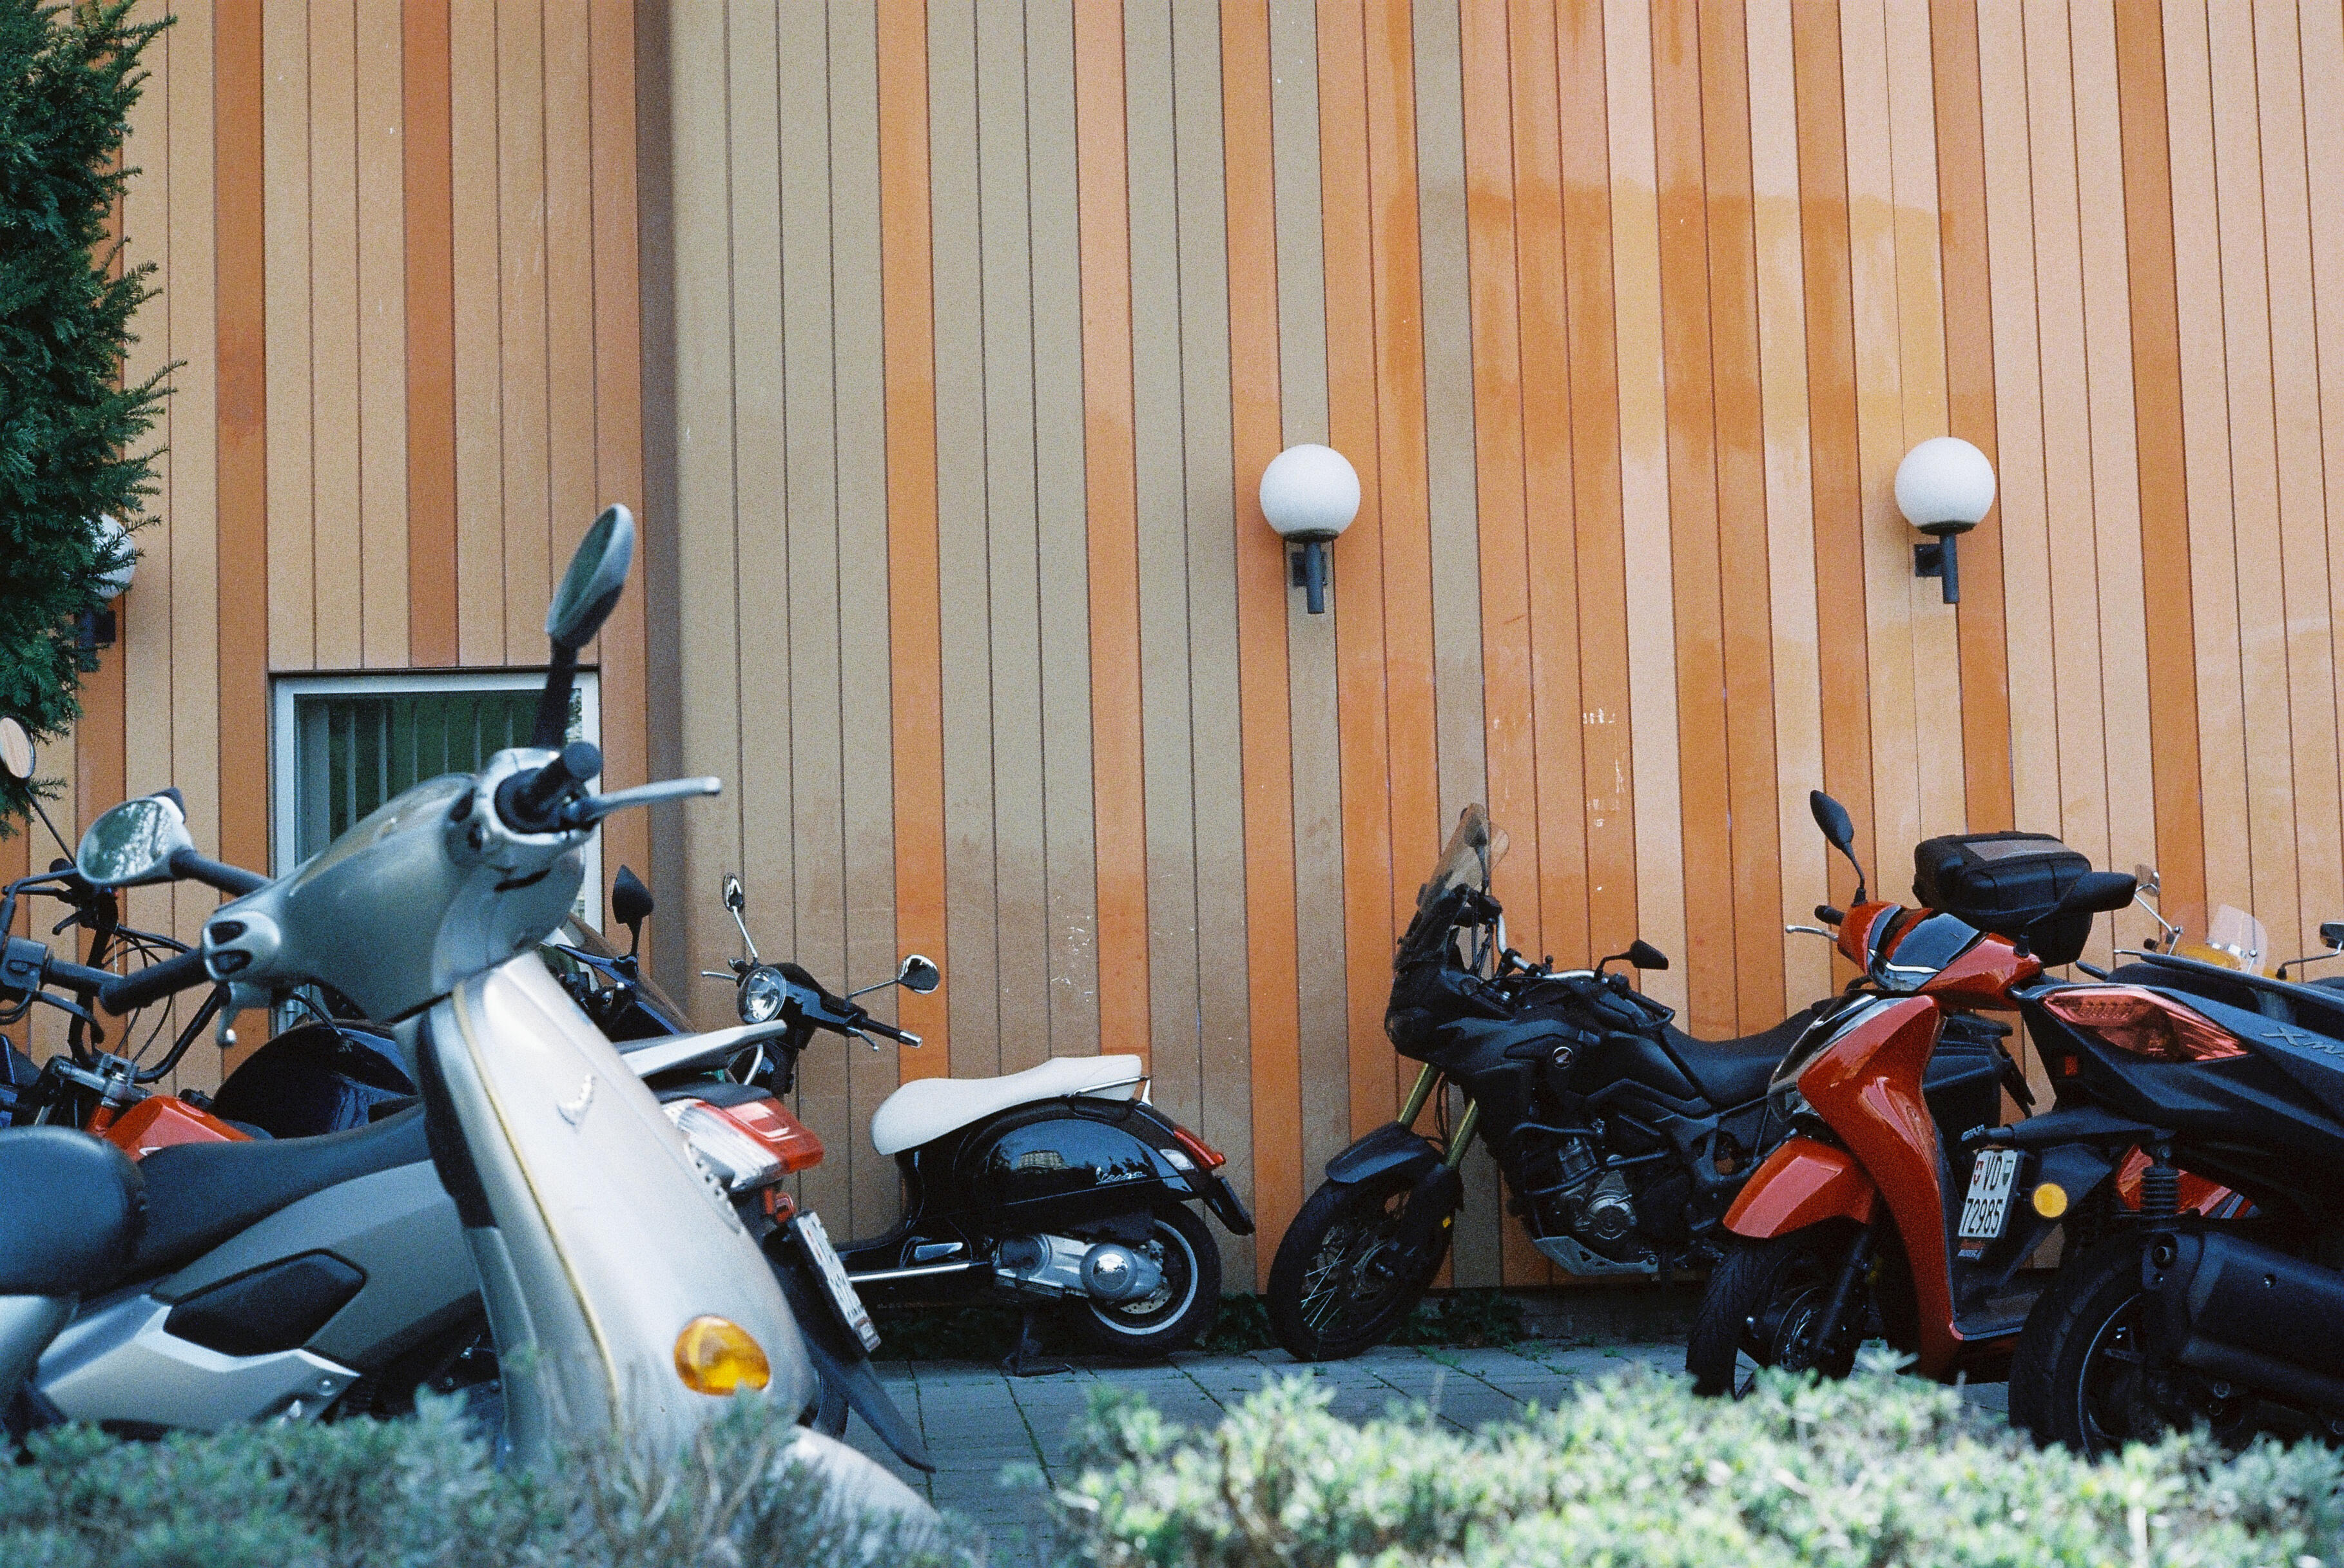
\includegraphics[width=\linewidth]{figures/raw-film.jpeg}
    %   \caption{Raw Film Image}
    % \end{subfigure}
    % \hfill
    % \begin{subfigure}[t]{.24\textwidth}
    %   \centering
    %   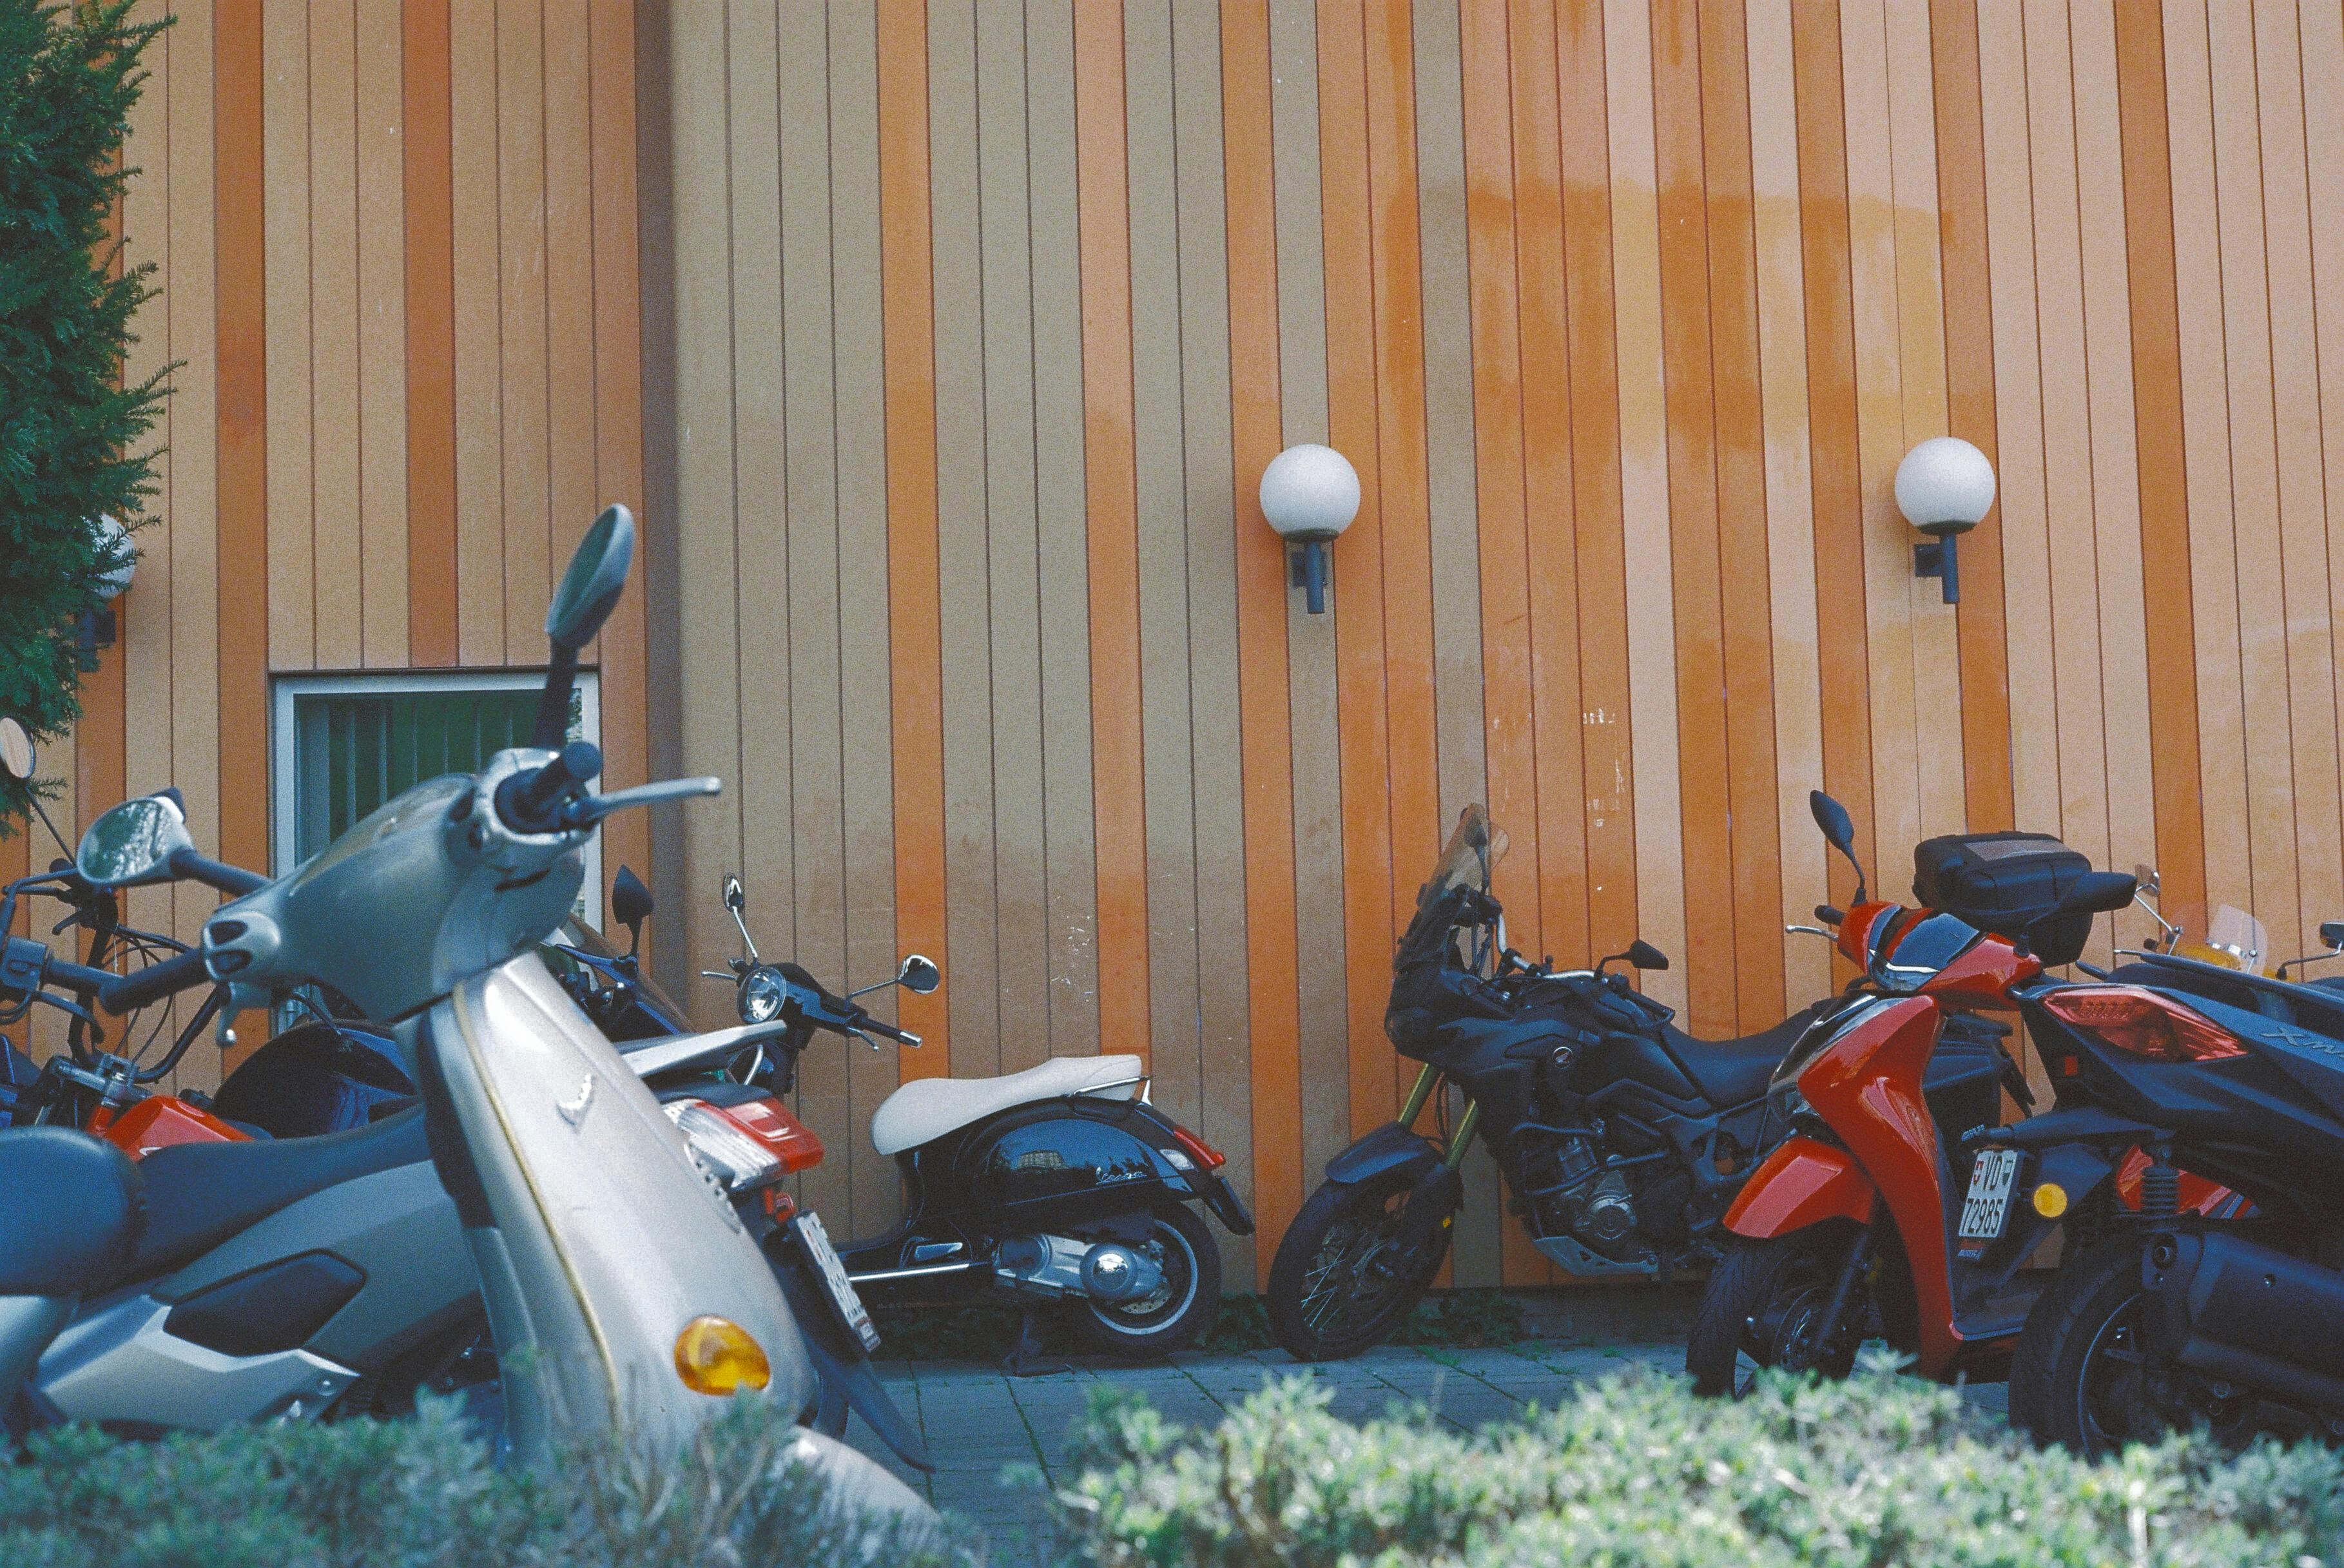
\includegraphics[width=\linewidth]{figures/processed-film.jpeg}
    %   \caption{Processed Film Image}
    % \end{subfigure}
    % \hfill
    % \begin{subfigure}[t]{.24\textwidth}
    %   \centering
    %   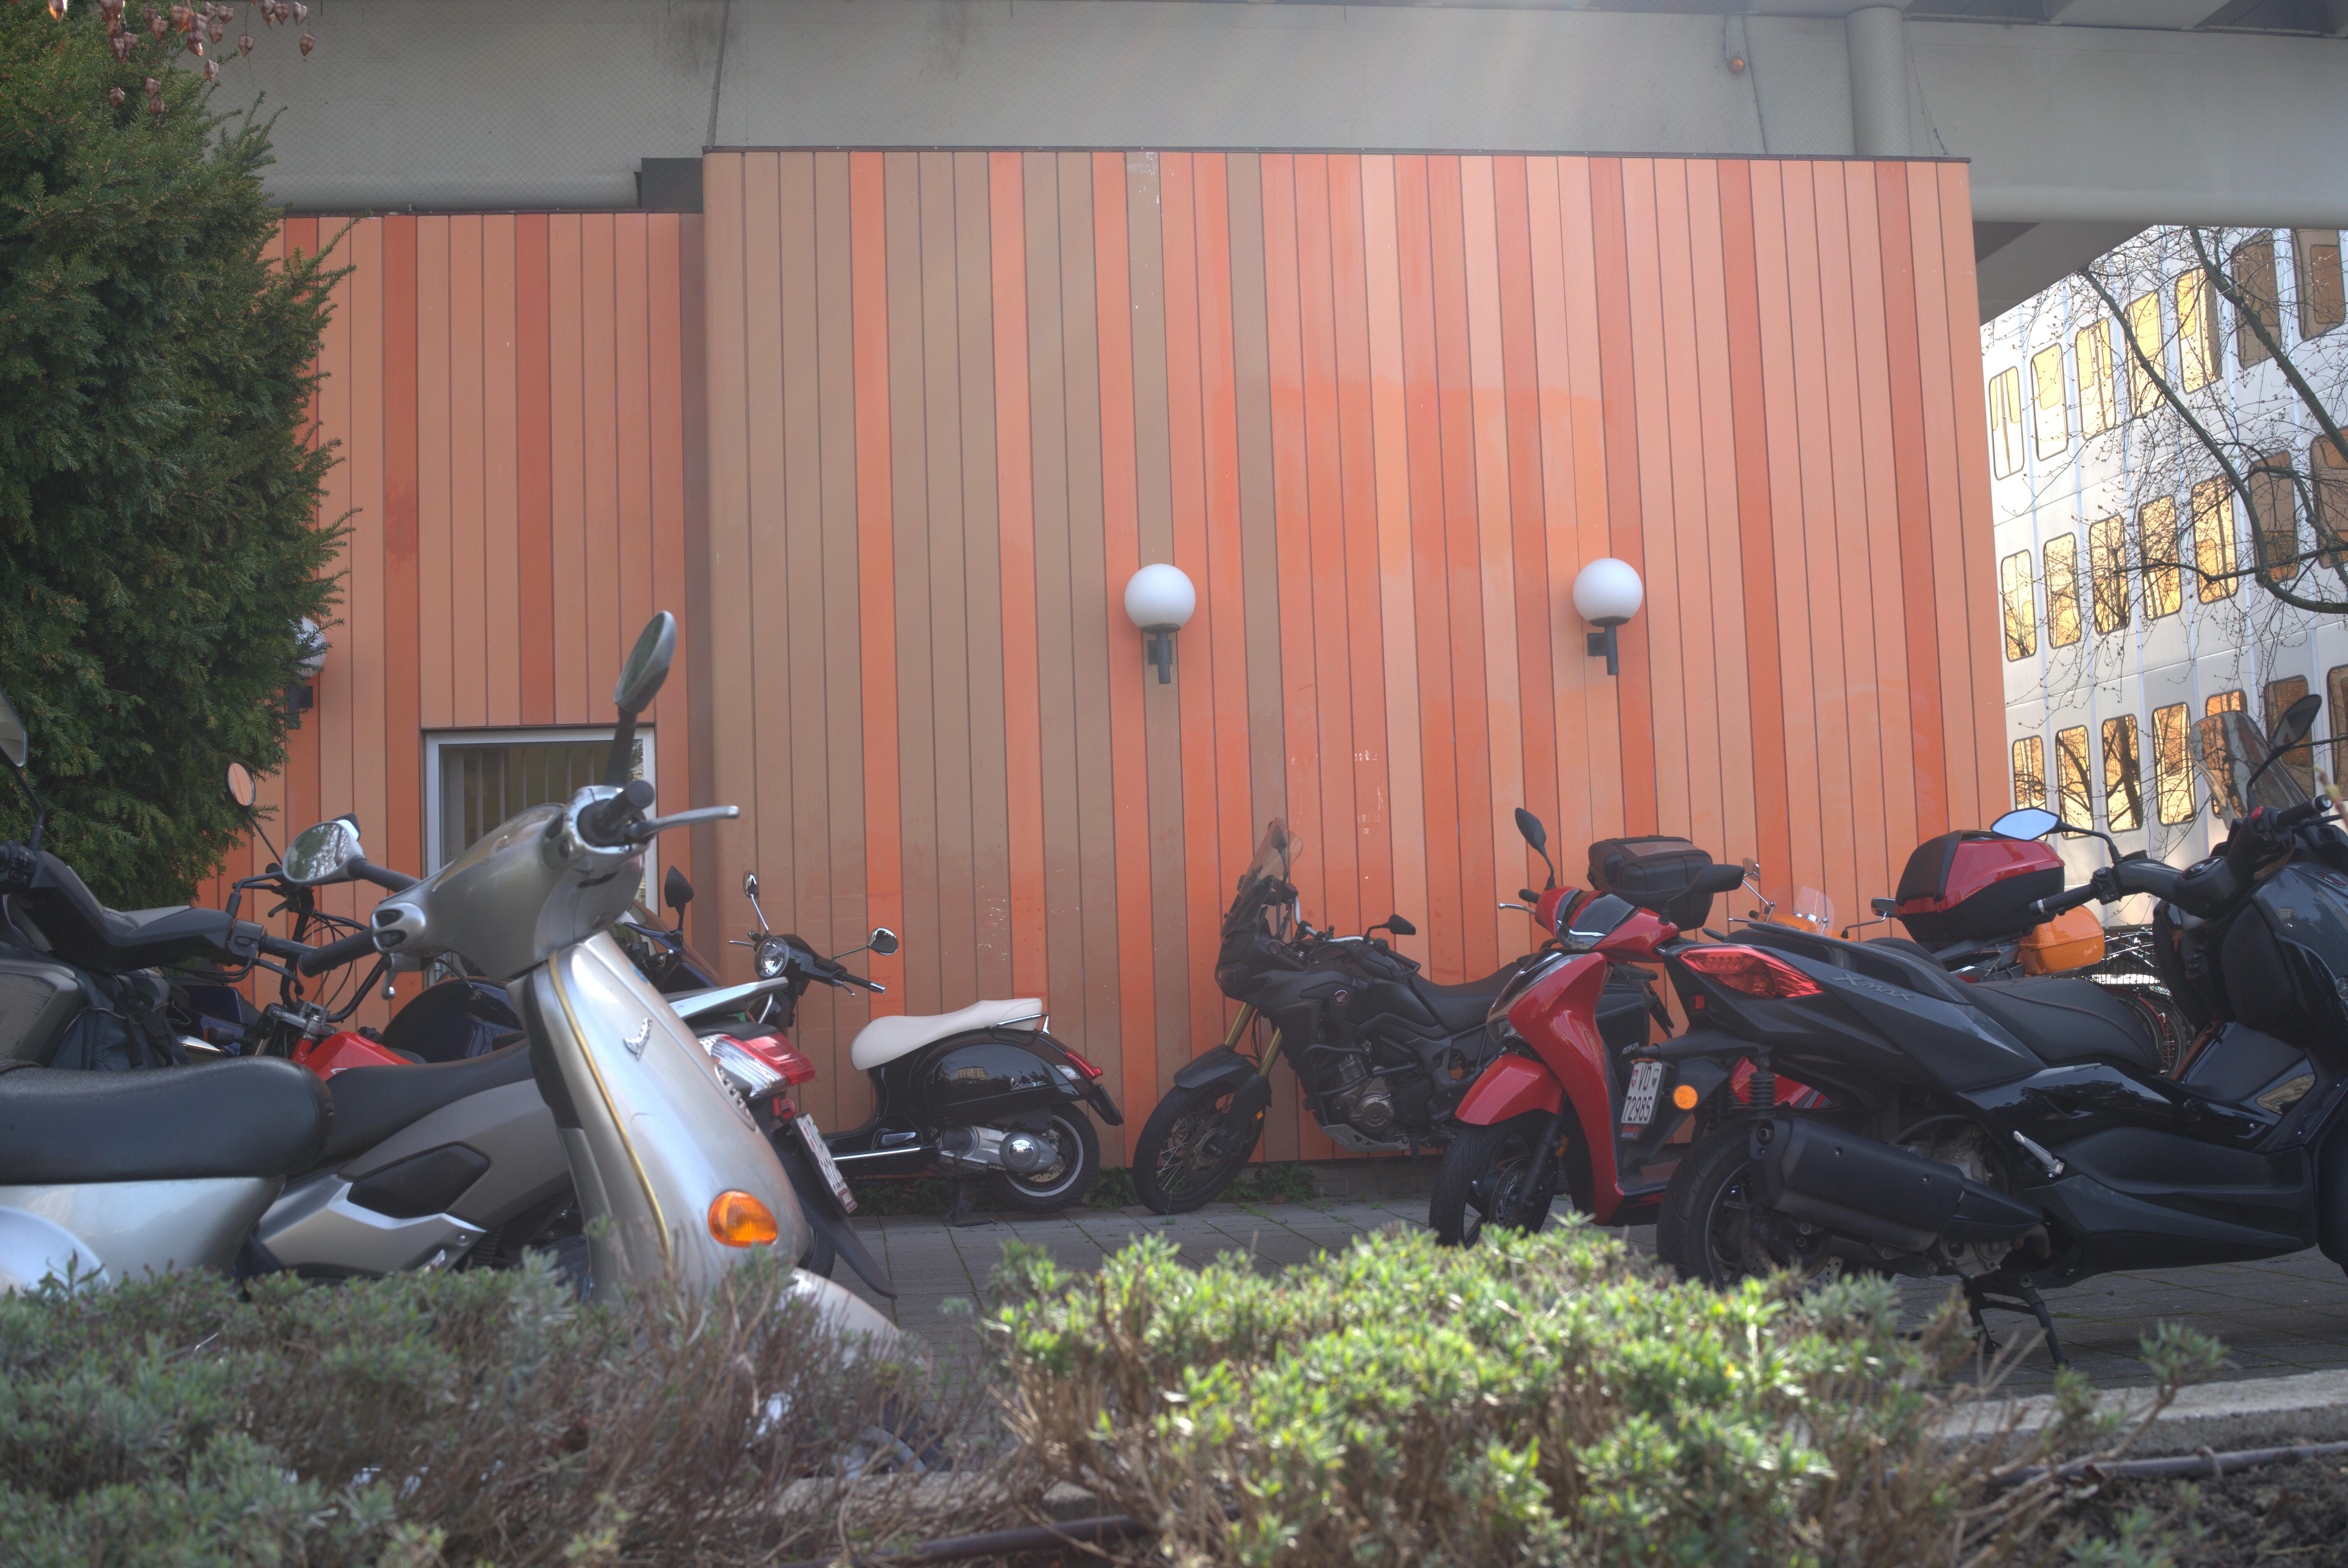
\includegraphics[width=\linewidth]{figures/raw-digital.jpeg}
    %   \caption{Raw Digital Image}
    % \end{subfigure}
    % \hfill
    % \begin{subfigure}[t]{.24\textwidth}
    %   \centering
    %   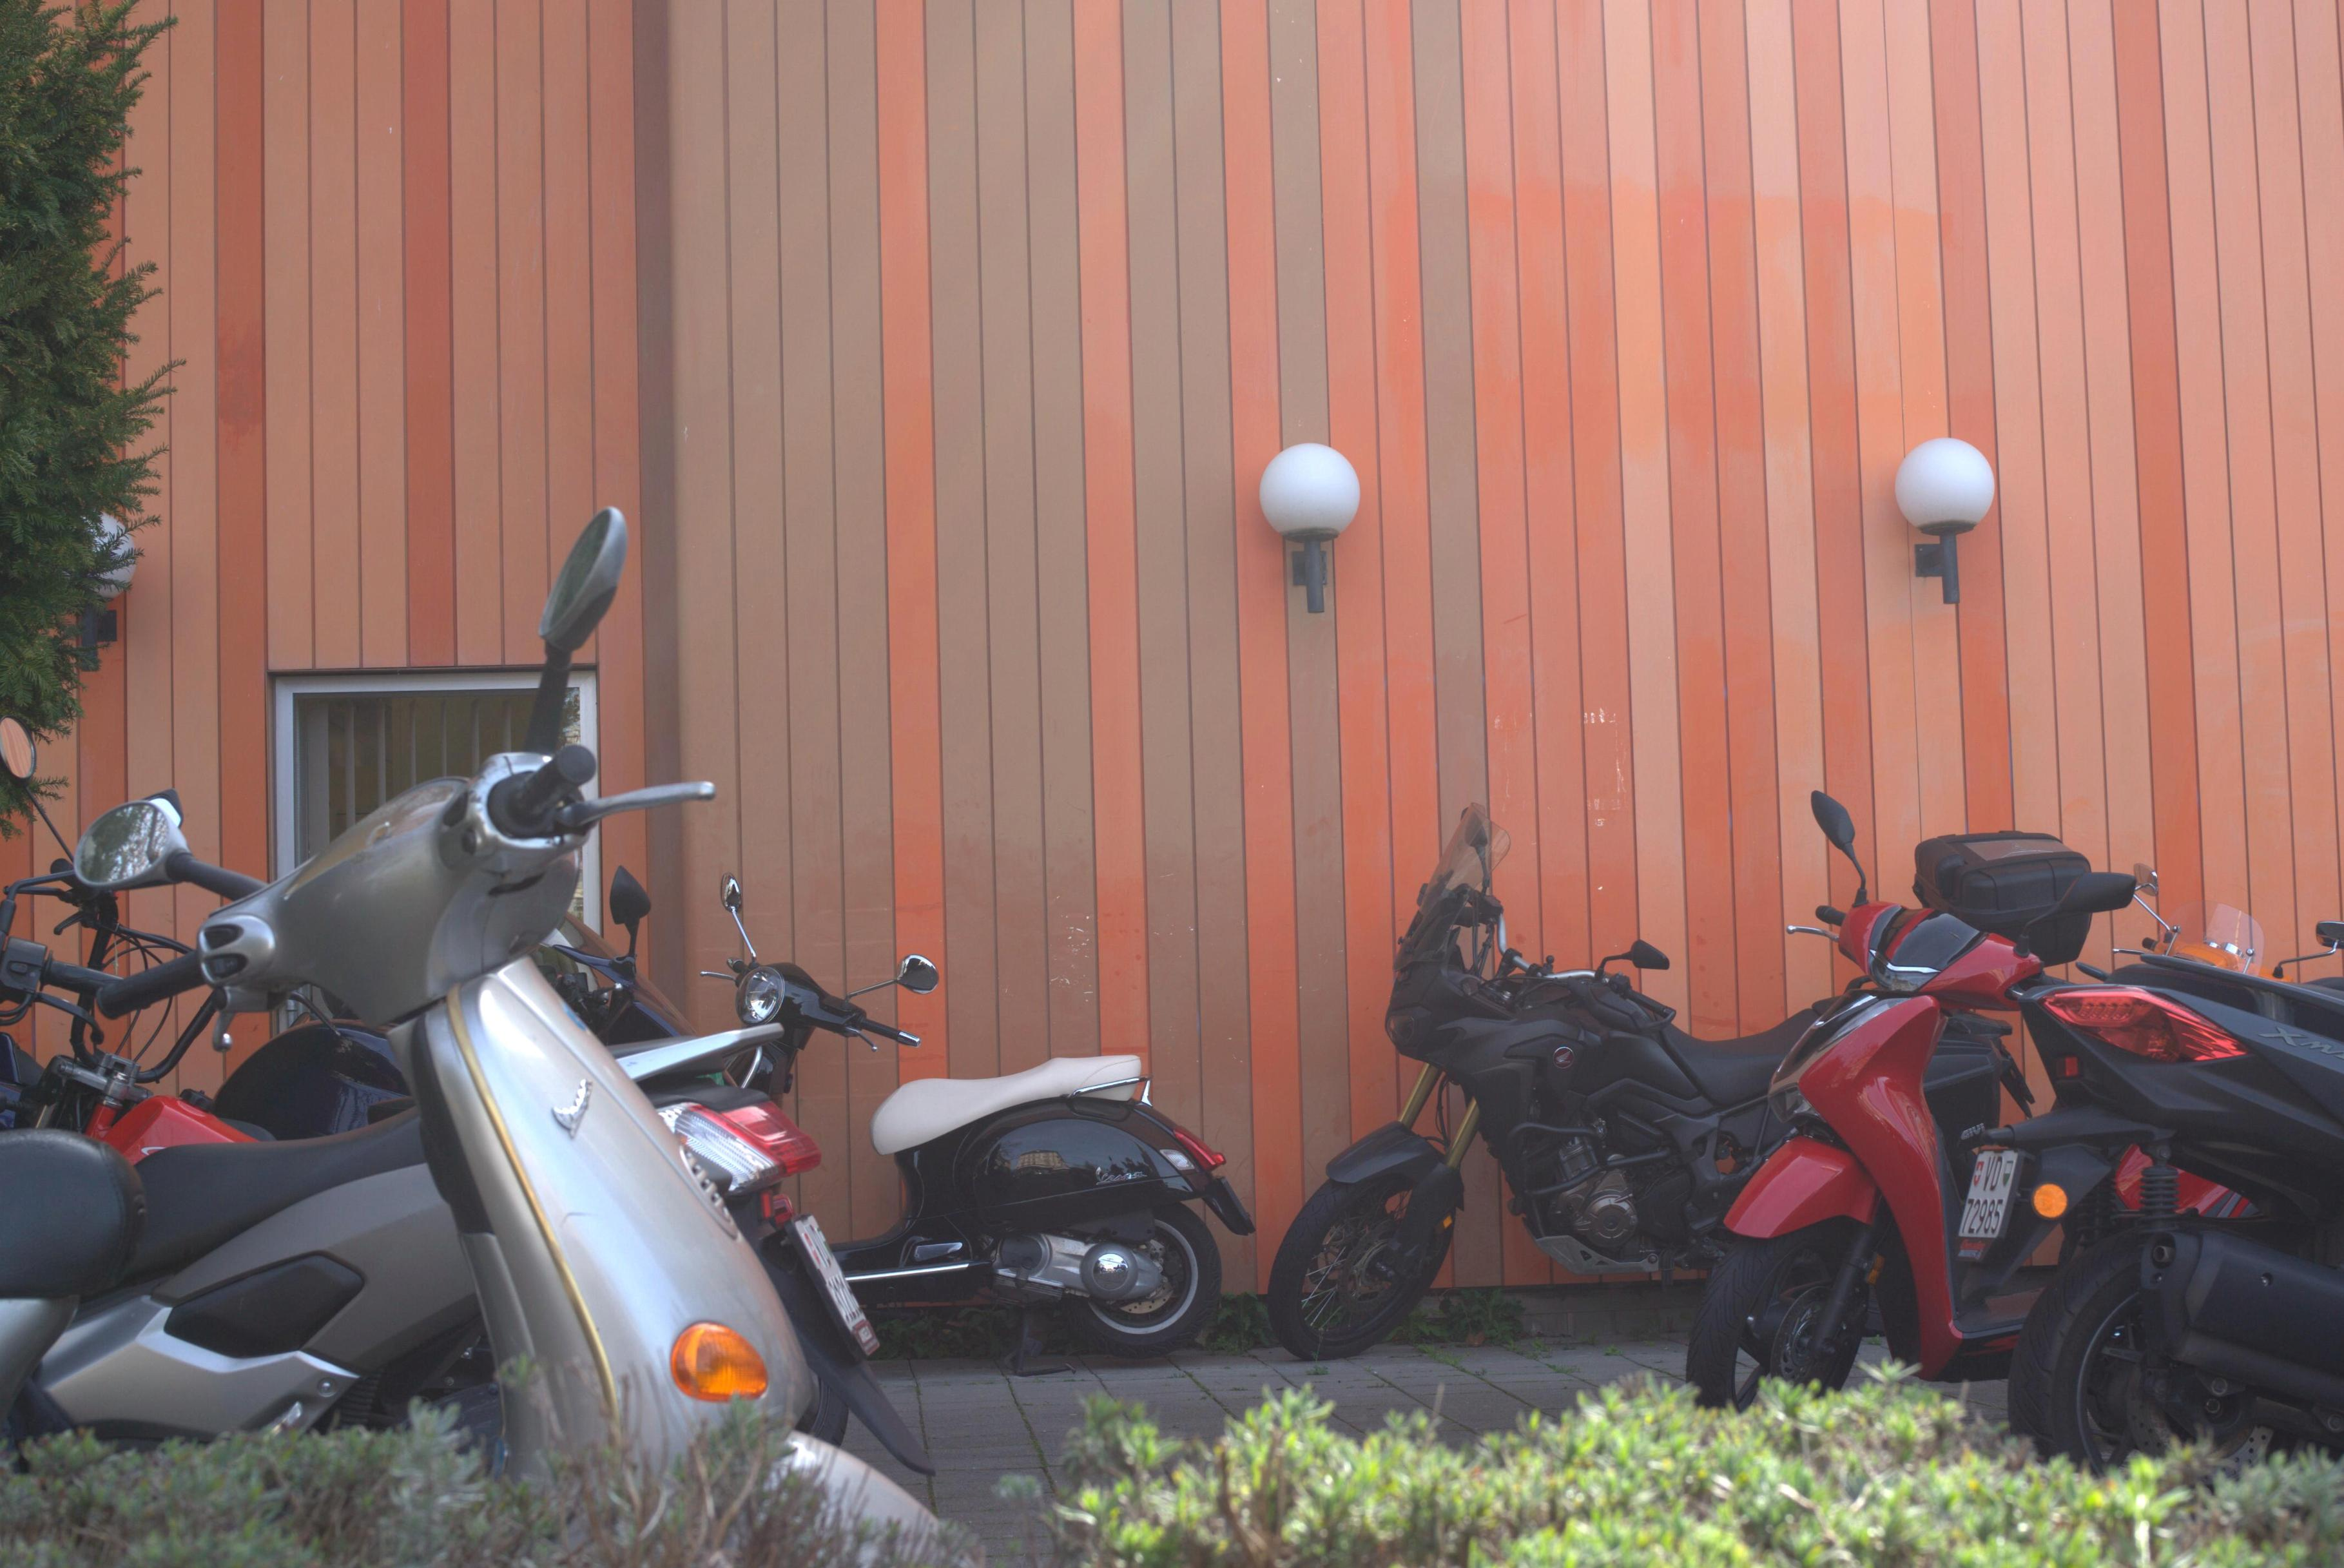
\includegraphics[width=\linewidth]{figures/processed-digital.jpeg}
    %   \caption{Processed Digital Image}
    % \end{subfigure}


    \begin{subfigure}[b]{0.49\textwidth}
      \centering
      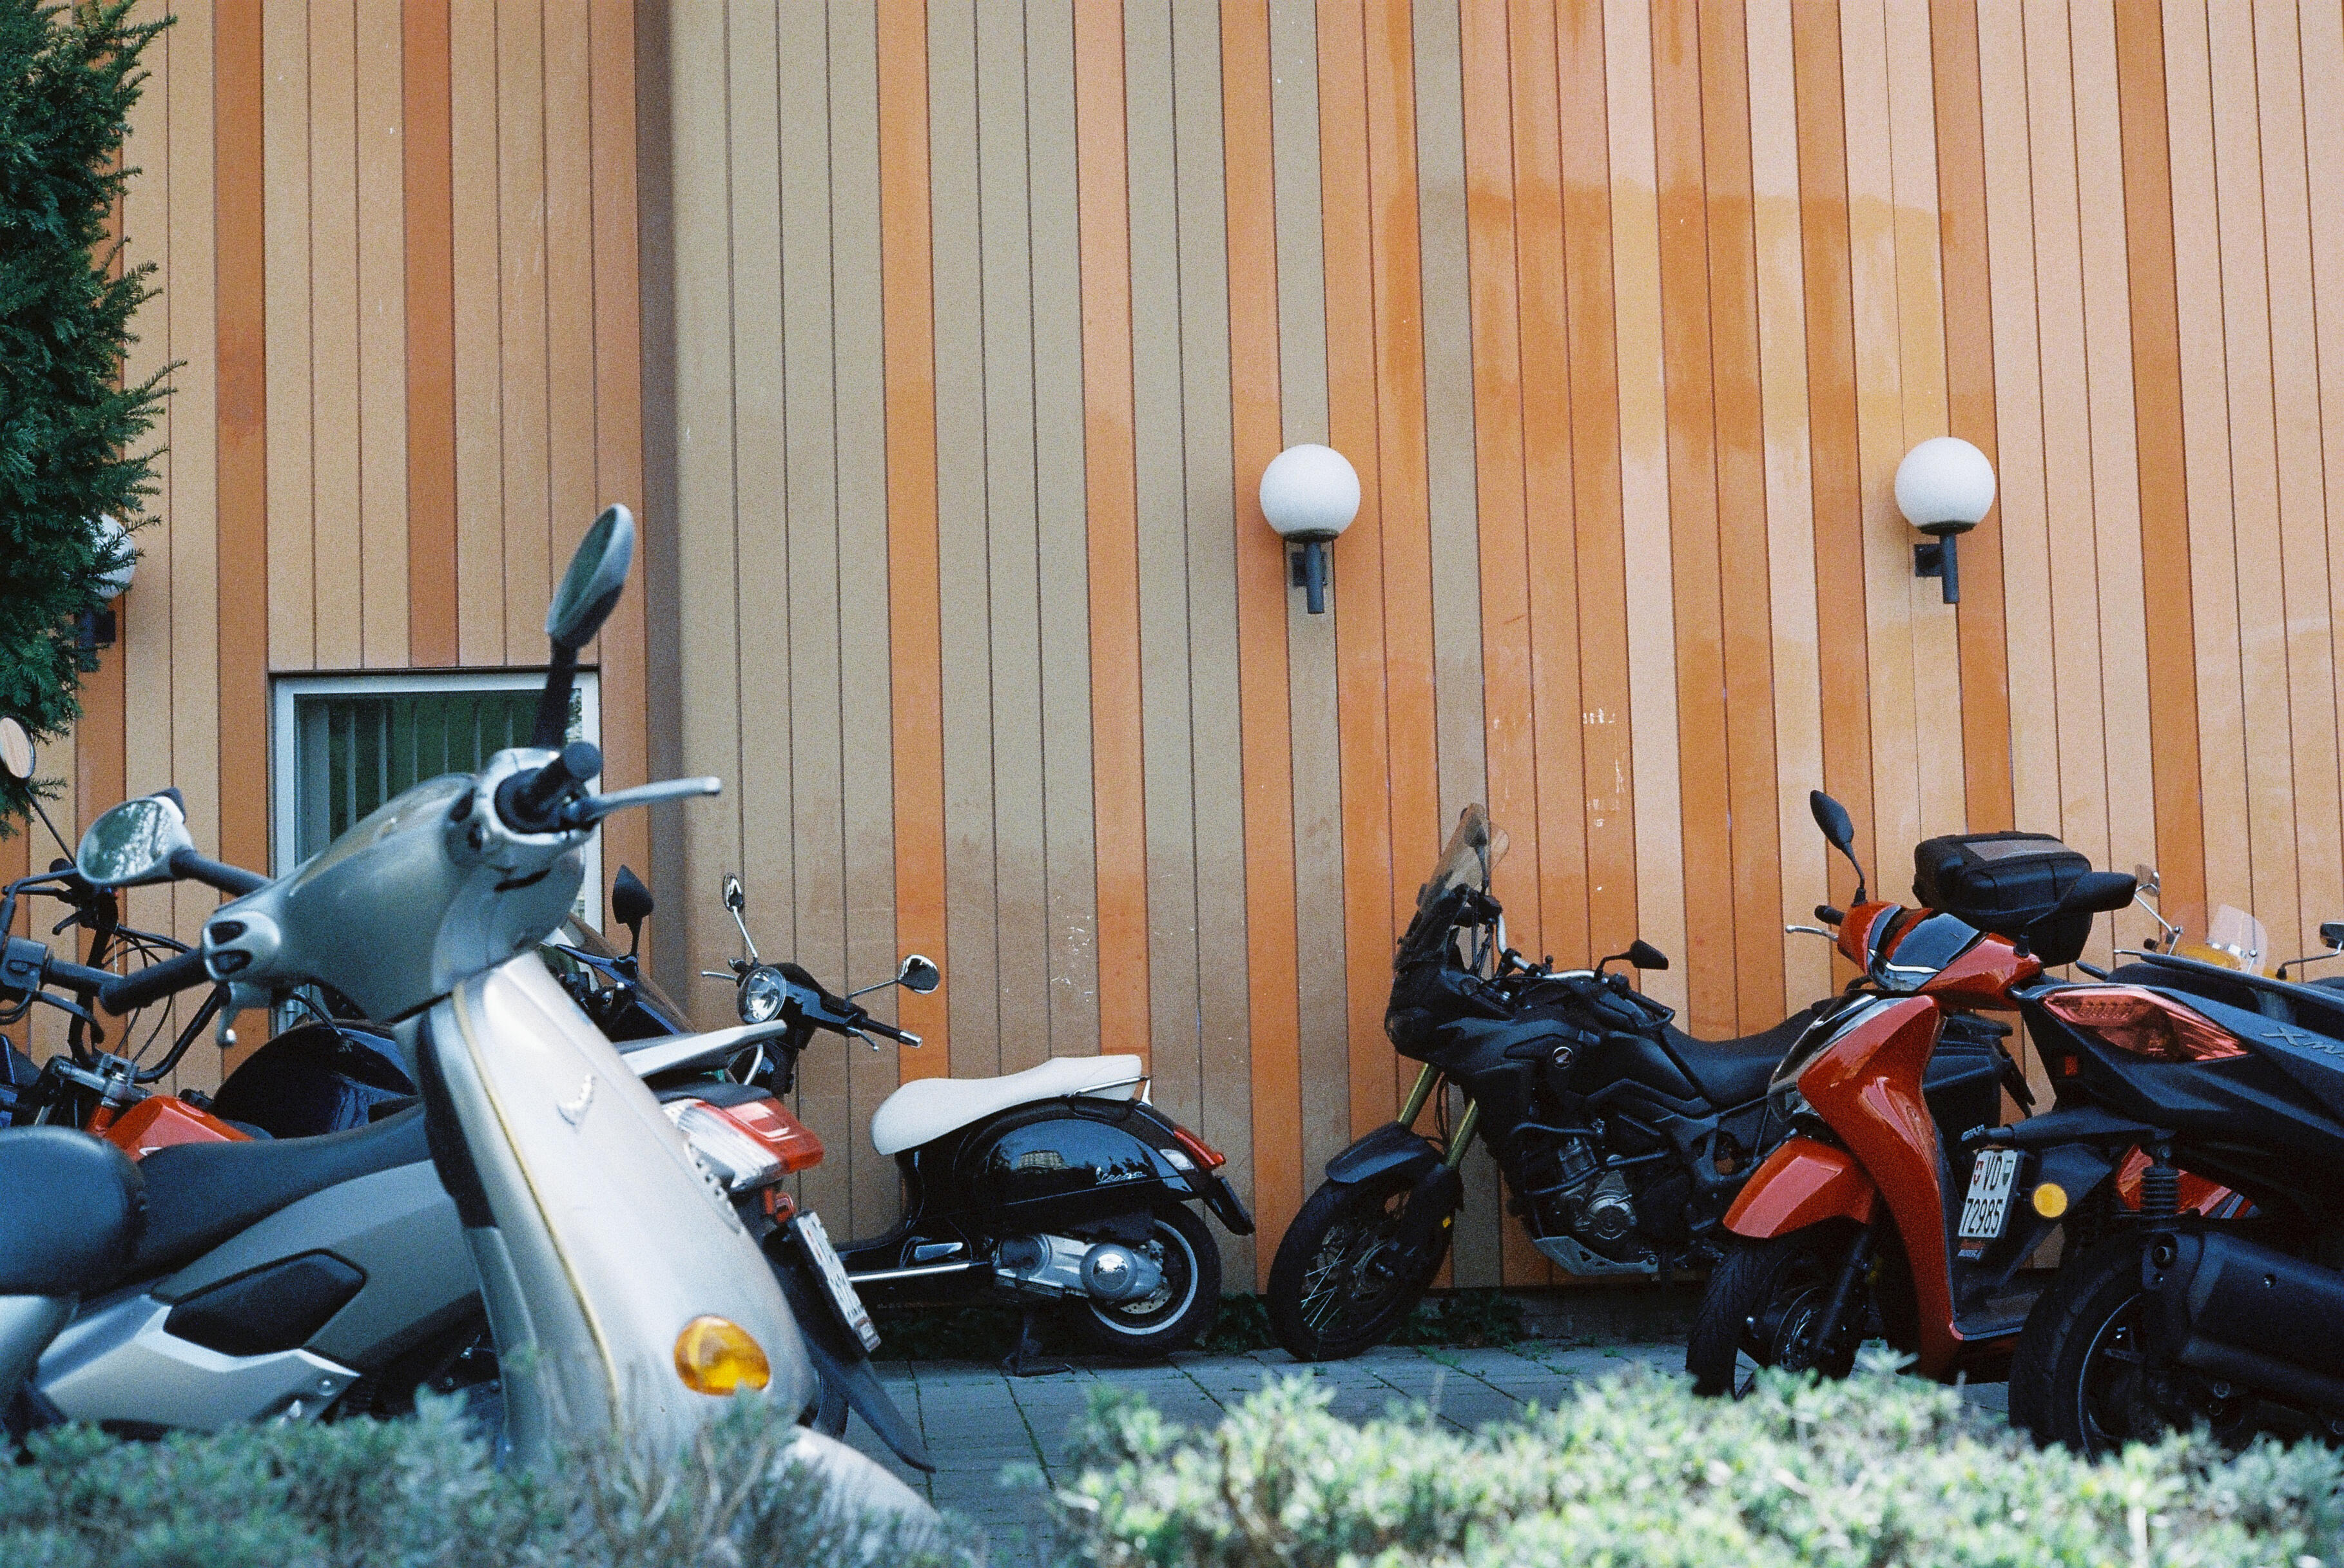
\includegraphics[width=0.49\textwidth]{figures/raw-film.jpeg}
      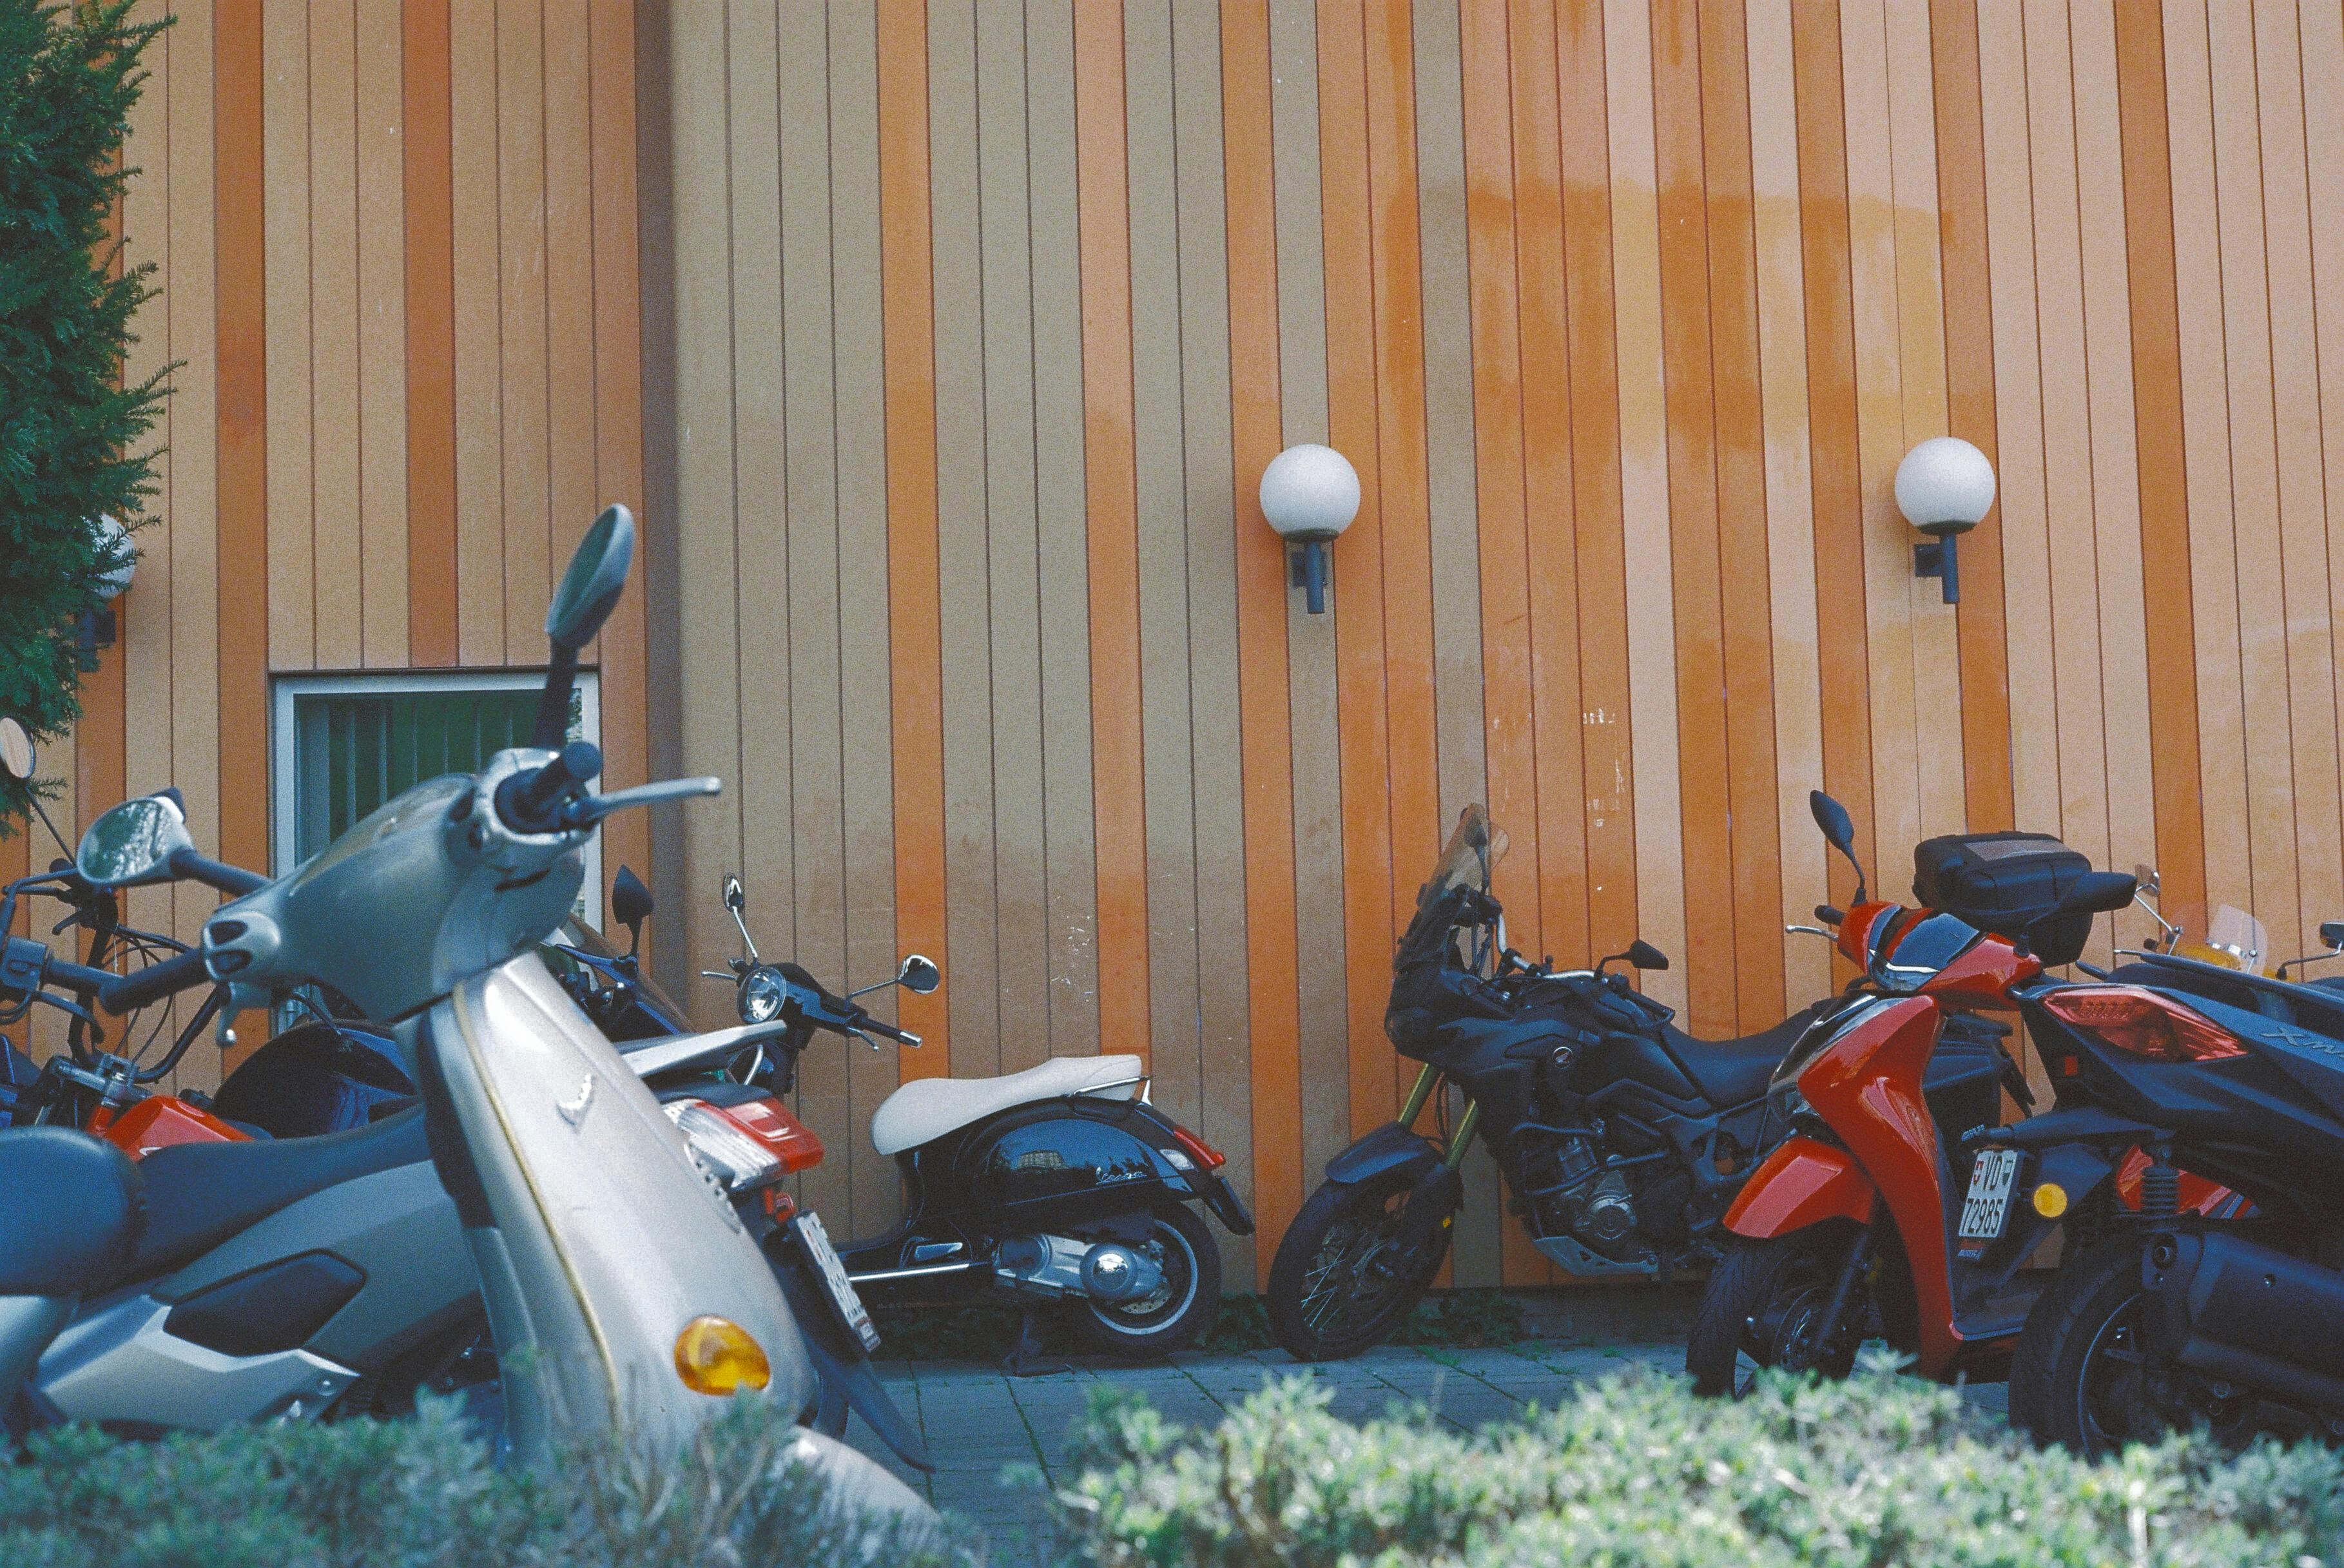
\includegraphics[width=0.49\textwidth]{figures/processed-film.jpeg}
      \captionsetup{justification=centering}
      \caption{Film: Raw (left) vs. Processed (right).} 
  \end{subfigure}
  \hfill
  \begin{subfigure}[b]{0.49\textwidth}
      \centering
      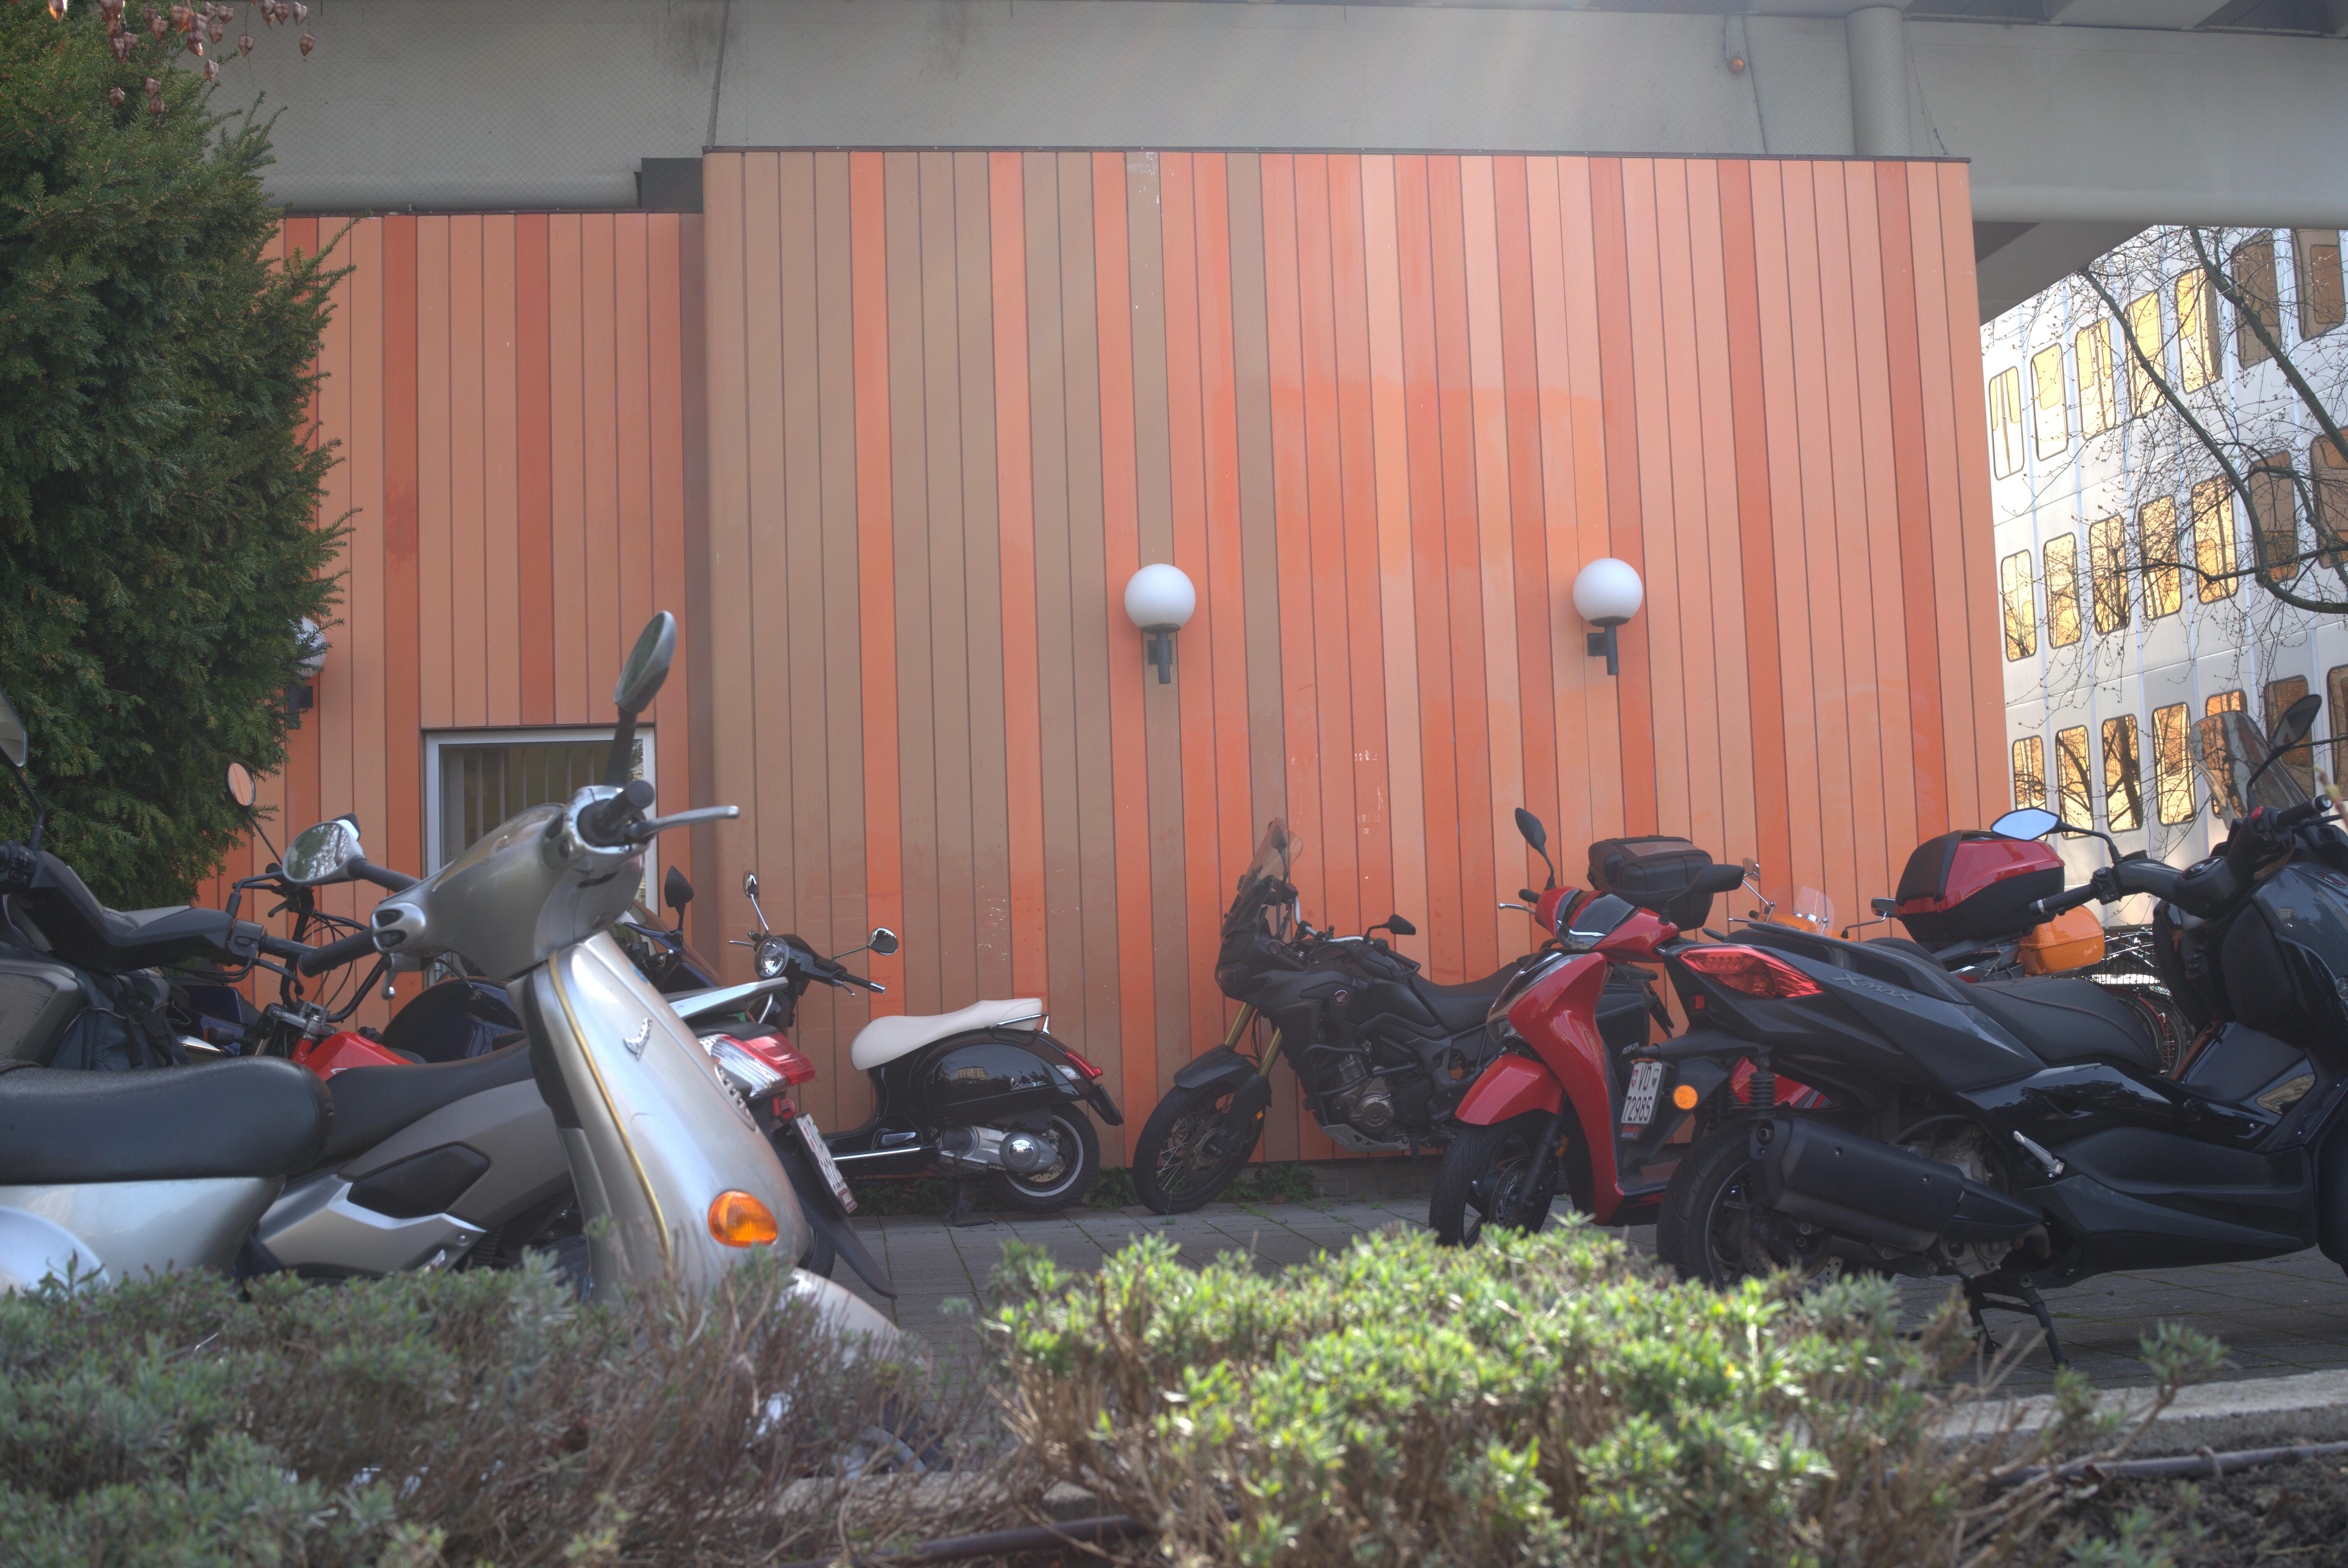
\includegraphics[width=0.49\textwidth]{figures/raw-digital.jpeg}
      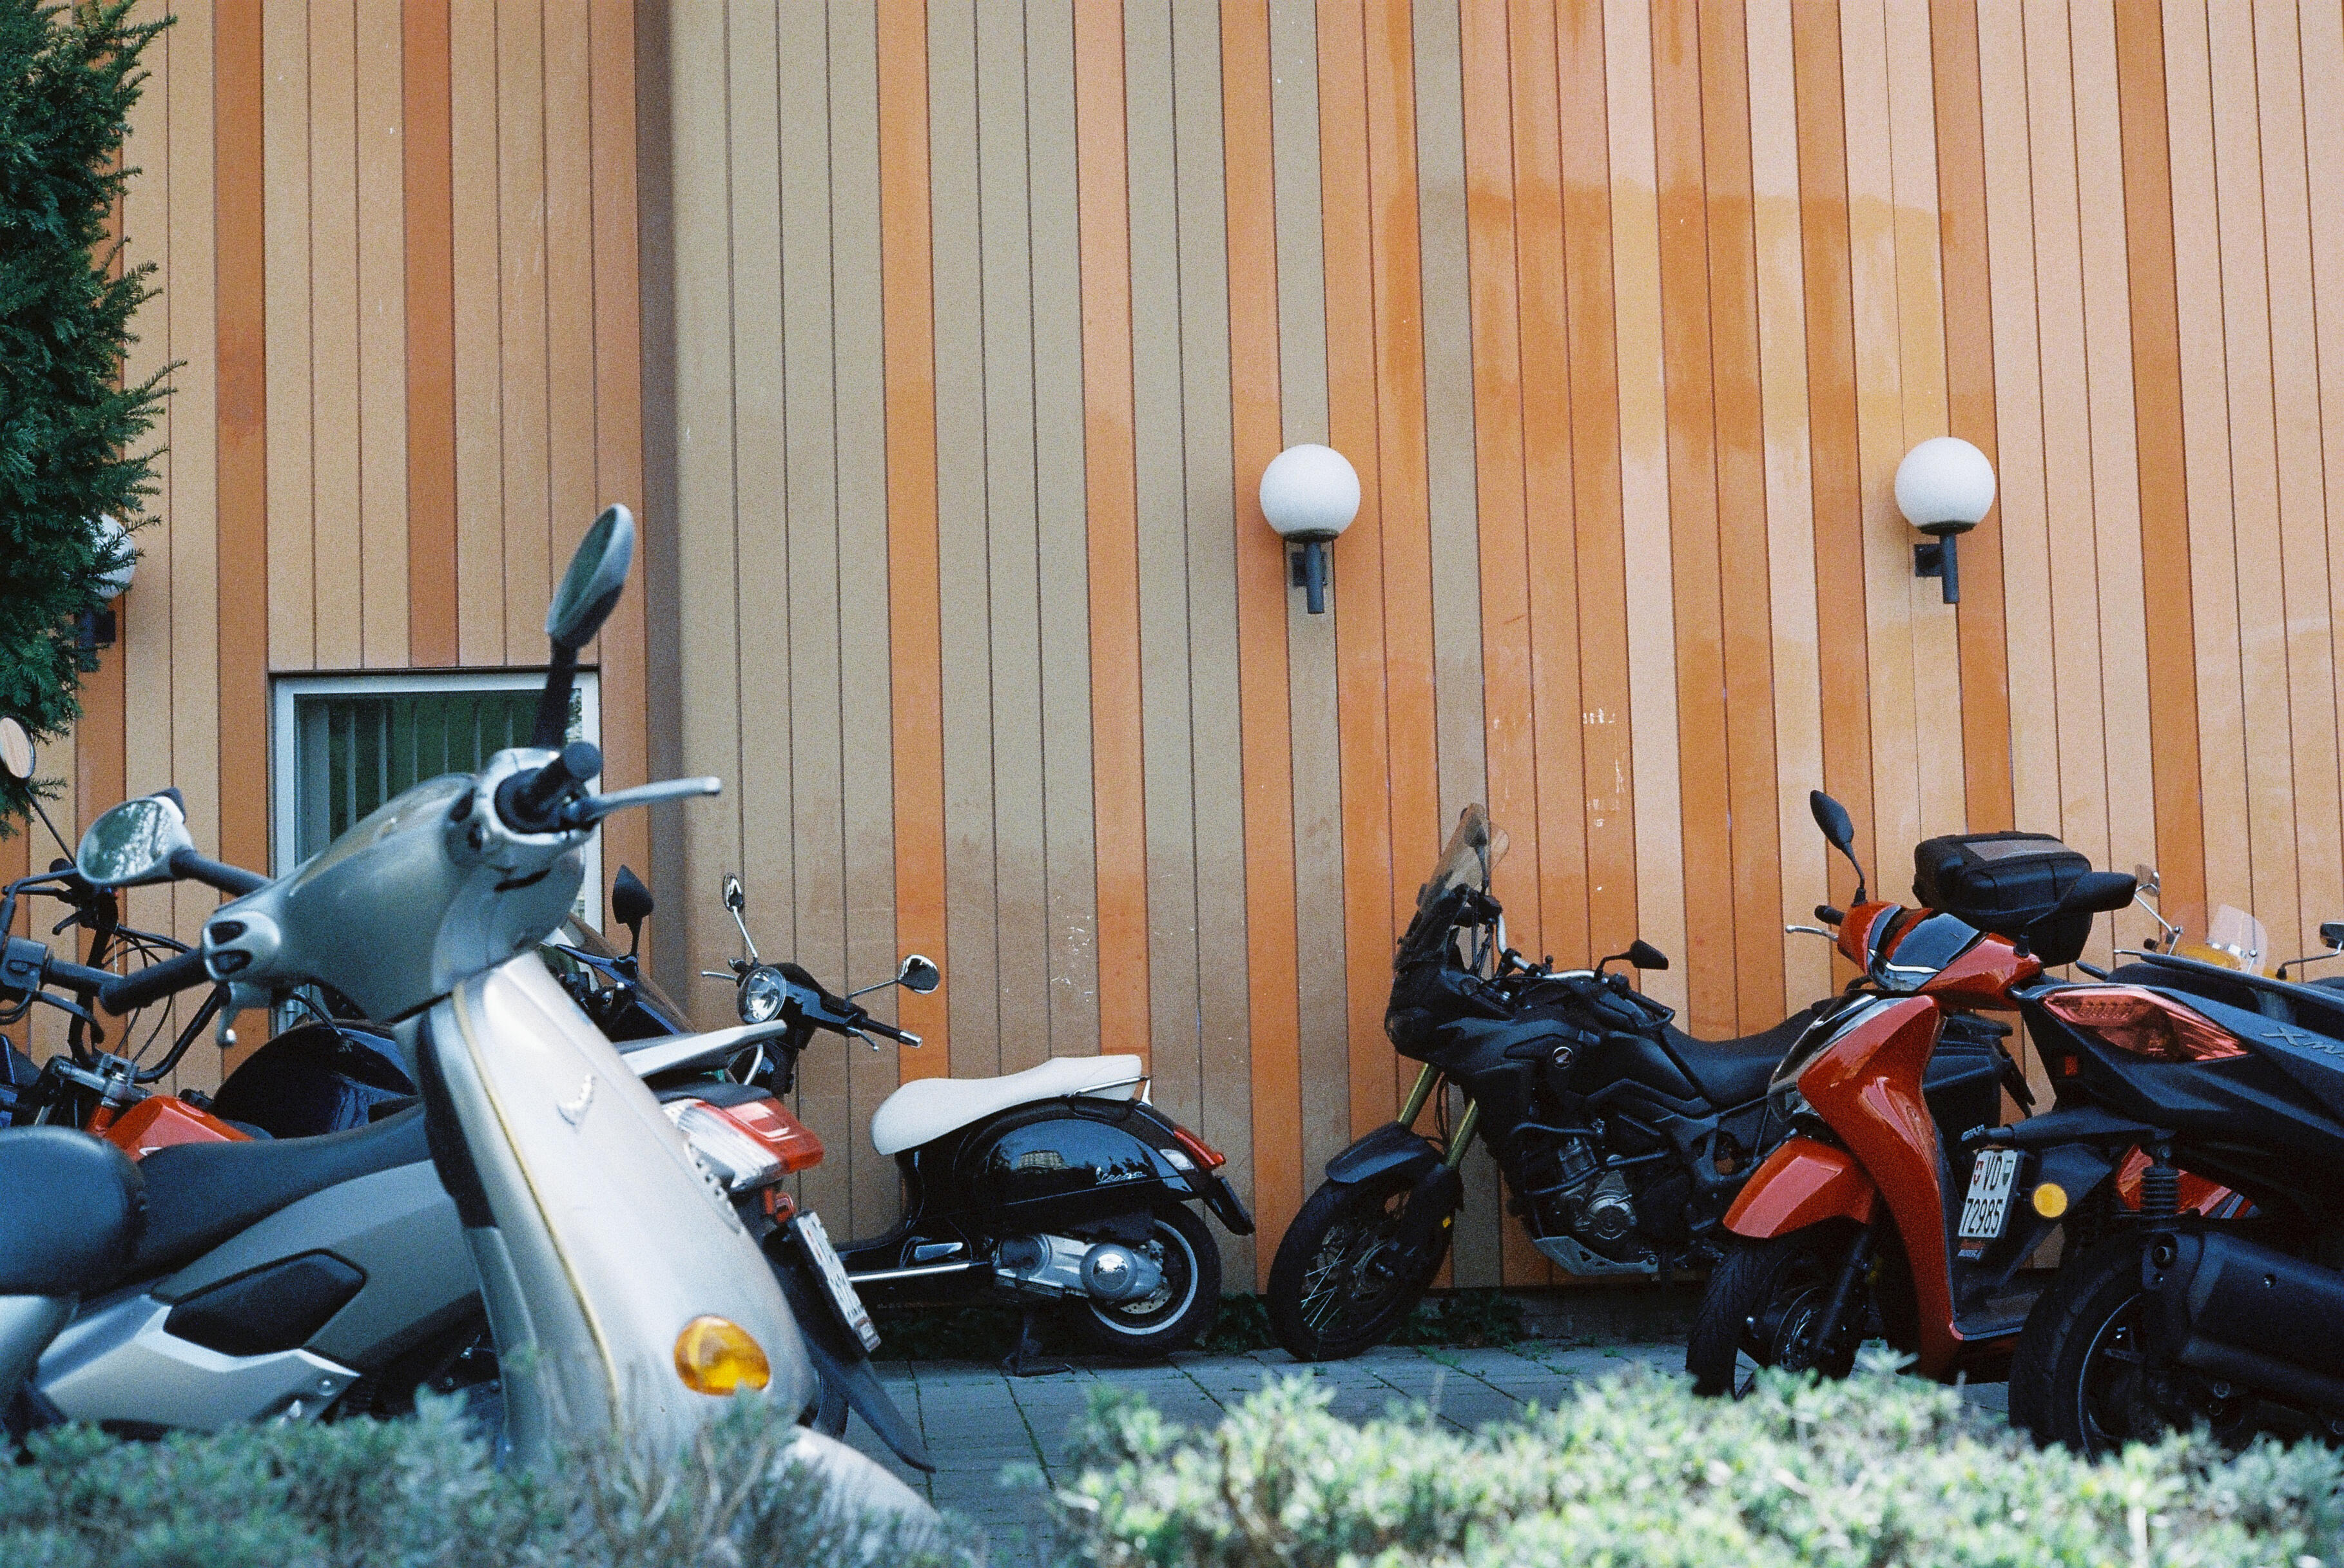
\includegraphics[width=0.49\textwidth]{figures/raw-film}
      \captionsetup{justification=centering}
      \caption{Digital: Raw (left) vs. Processed (right).}
  \end{subfigure}

    \caption{\textbf{Dataset Preprocessing.} Example of a raw and processed image pair. We can see the luminance alignment in the film image (a) and the spatial alignment in the digital image (b).}
    \label{fig:data-preprocessing}
\end{figure}

% Maybe talk about data augmentation (horizontal/ vertical flips, brightness adjustment and blur)
% We didn't do this for our final runs, so no.